%% $Id: paper.tex 59236 2018-04-25 08:28:29Z cfrioux $
%% $HeadURL: https://svn.cs.uni-potsdam.de/svn/reposWV/Papers/ExpansionAlg/trunk/paper.tex $

\documentclass{new_tlp}

\usepackage[utf8]{inputenc}
\usepackage{microtype}
\usepackage{xparse,xifthen}
\usepackage{natbib}
\usepackage{amsmath,amssymb}
\let\proof\relax
\let\endproof\relax
\usepackage{amsthm}%,thmtools,environ}
\usepackage{url}
\usepackage{listings}
\usepackage[dvipsnames]{xcolor}
\usepackage{tikz}
\usepackage{slashbox}

\makeatletter
\let\O@argtabularcr\@argtabularcr
\def\O@xtabularcr{\@ifnextchar[\O@argtabularcr{\ifnum 0=`{\fi}\cr}}
\let\O@tabacol\@tabacol
\let\O@tabclassiv\@tabclassiv
\let\O@tabclassz\@tabclassz
\let\O@tabarray\@tabarray
\def\author@tabular{\authorsize\def\@halignto{}\@authortable}
\let\endauthor@tabular=\endtabular
\def\author@tabcrone{{\ifnum0=`}\fi\O@xtabularcr\affilsize\itshape
 \let\\=\author@tabcrtwo\ignorespaces}
\def\author@tabcrtwo{{\ifnum0=`}\fi\O@xtabularcr[-3\p@]\affilsize\itshape
 \let\\=\author@tabcrtwo\ignorespaces}
\def\@authortable{\leavevmode \hbox \bgroup $\let\@acol\O@tabacol
 \let\@classz\O@tabclassz \let\@classiv\O@tabclassiv
 \let\\=\author@tabcrone \ignorespaces \O@tabarray}
\makeatother


\usepackage{xcolor,colortbl}
\usepackage{xintexpr, xinttools}
\usepackage{caption}
%\usepackage{colortbl}

\lstset{numberbychapter=false,basicstyle=\ttfamily,captionpos=b,floatplacement=t}

\renewcommand{\topfraction}{1}
\renewcommand{\bottomfraction}{1}
\renewcommand{\textfraction}{0}

\newcommand{\review}[1]{{\textcolor{red}{#1}}}

\newcommand{\gringo}{\textit{gringo}}
\newcommand{\clasp}{\textit{clasp}}
\newcommand{\clingo}{\textit{clingo}}
\newcommand{\asprin}{\textit{asprin}}
\newcommand{\asap}{\textit{teaspoon}}
\newcommand{\piclasp}{\textit{piclasp}}

\newcommand{\code}[1]{\lstinline[basicstyle=\ttfamily]{#1}}

\newcommand{\lw}[1]{\smash{\lower1.ex\hbox{#1}}}
\newcommand{\llw}[1]{\smash{\lower3.ex\hbox{#1}}}

%\newcommand{\dataCL}[5]{%
%  \code{#1} & #3 & #5 & #4
%}
%\newcommand{\dataCS}[5]{%
%  #3 & #5 & #4
%}

\newenvironment{tableC}{%
  \scriptsize
  \tabcolsep = 0.6mm
  \begin{tabular}[t]{l|rlr|rlr|rlr|rlr|rlr}\hline
    \multicolumn{1}{l|}{\llw{Instance}} &
    \multicolumn{3}{c|}{UD1} &
    \multicolumn{3}{c|}{UD2} &
    \multicolumn{3}{c|}{UD3} &
    \multicolumn{3}{c|}{UD4} &
    \multicolumn{3}{c}{UD5} \\
    & 
    \multicolumn{1}{c}{Best} & & \multicolumn{1}{c|}{\emph{tea-}} & 
    \multicolumn{1}{c}{Best} & & \multicolumn{1}{c|}{\emph{tea-}} & 
    \multicolumn{1}{c}{Best} & & \multicolumn{1}{c|}{\emph{tea-}} & 
    \multicolumn{1}{c}{Best} & & \multicolumn{1}{c|}{\emph{tea-}} & 
    \multicolumn{1}{c}{Best} & & \multicolumn{1}{c}{\emph{tea-}} \\
    & 
    known & & \emph{spoon} & 
    known & & \emph{spoon} & 
    known & & \emph{spoon} & 
    known & & \emph{spoon} & 
    known & & \emph{spoon} \\
    \hline
  }{%
    \hline
  \end{tabular}
}

\newenvironment{tableB}{%
  \scriptsize
  \tabcolsep = 0.7mm
%  \begin{tabular}[t]{|l|c|r|l|l|l|}\hline
  \begin{tabular}[t]{lcrlll}\hline
    Instance &
    Formulation &
    Time (sec.)\\
    \hline
  }{%
    \hline
  \end{tabular}
}
\newenvironment{tableL}{%
  \scriptsize
  \tabcolsep = 0.7mm
  \begin{tabular}[t]{l|rrrrrrrr|r}\hline
    \lw{Instance} &
    \lw{Time (sec.)} &
    \multicolumn{6}{c}{The best utility vector} &
    The sum of  &
    The best of basic\\
    &
    &
    $(S_1,$ & $S_4,$ & $S_2,$ & $S_7,$ & $S_6,$ & $S_3)$ &
    utility vector &
    and optimized \\
    \hline
  }{%
    \hline
  \end{tabular}
}

%%% Local Variables:
%%% mode: latex
%%% TeX-master: "paper"
%%% End:


\allowdisplaybreaks

\title{Hybrid Metabolic Network Completion}

\author[C.~Frioux, T.~Schaub, S.~Schellhorn, A.~Siegel, and P.~Wanko]{%
  Clémence Frioux
  \\
  Univ Rennes, Inria, CNRS, IRISA F-35000 Rennes, France
  \and
  Torsten Schaub%  orsten \thanks{Affiliated with the
                          %     School of Computing Science at
                          %     Simon Fraser University,
                          %     Burnaby, Canada,
                          %     and the
                          %     Institute for Integrated and Intelligent Systems
                          %     at
                          %     Griffith University,
                          %     Brisbane, Australia.}
  \\
  Inria, Rennes, France \ and \ Universit\"at Potsdam, Germany
  \and
  Sebastian Schellhorn
  \\
  Universit\"at Potsdam, Germany
  \and
  Anne Siegel
  \\
  Univ Rennes, Inria, CNRS, IRISA F-35000 Rennes, France
  \and
  Philipp Wanko
  \\
  Universit\"at Potsdam, Germany} %


\begin{document}

\maketitle
%\begin{abstract}
%	The design space for highly complex system level specifications of embedded systems is enormous as tasks may be mapped to different resources and messages may be routed over several links of the hardware platform. 
%	Furthermore, highly constrained requirements lead to many infeasible solutions that have to be sorted out. \emph{\ac{ASP}} in combination with variant background theories (\emph{\ac{ASPmT}}) has been shown to cope with such requirements very efficiently. However, especially in system level design, a fast \emph{\ac{DSE}} including optimization is crucial in order to steer the development towards optimal design points. In this paper, we therefore propose to couple the highly efficient constraint solving capabilities of \ac{ASP} with a \ac{DSE} including \emph{multi-objective optimization} in an additional background theory. Utilizing the possibility to work on \emph{partial assignments}, \ac{ASPmT} is able to prune entire infeasible and dominated regions from the search space early in the decision process. In the experimental section, we present and compare variant approaches and domain specific heuristics.
%\end{abstract}

\begin{abstract}
	An efficient \emph{\ac{DSE}} is imperative for the design of modern, highly complex embedded systems in order to steer the development towards optimal design points. The early evaluation of design decisions at system-level abstraction layer helps to find promising regions for subsequent development steps in lower abstraction levels by diminishing the complexity of the search problem. In recent works, symbolic techniques, especially \ac{ASPmT}, have been shown to find feasible solutions of highly complex system-level synthesis problems with non-linear constraints very efficiently. In this paper, we present a novel approach to a holistic system-level \ac{DSE} based on \ac{ASPmT}. To this end, we include additional background theories that concurrently guarantee compliance with hard constraints and perform the simultaneous optimization of several design objectives. %First experimental results show the applicability of our approach. %for large optimization of up to 170 tasks mapped to 3-dimensional hardware platforms. Furthermore, it outperforms current multi-objective optimization strategies of \ac{ASP} with respect to both diversity and convergence of found solutions.   %We present and investigate several strategies that show the applicability of our approach even for large problem instances. 
	We implement and compare our approach with a state-of-the-art preference handling framework for \ac{ASP}. Experimental results indicate that our proposed method produces better solutions with respect to both diversity and convergence to the true Pareto front.
\end{abstract}
\section{Introduction}
\label{sec:introduction}
%In order to cope with the ever-increasing complexity of embedded systems, system level description are utilized to diminish the complexity of finding potentially good solutions which can then be used as initial starting points for further optimization in lower abstraction levels. On system level, applications are composed of granular tasks that exchange information over communication messages and form dependency relations between each other. The hardware architecture contains heterogeneous processing elements (e.g.~CPU, DSP, GPU) as well as a communication infrastructure like routers and links. Yet, the design space for such system level specifications of embedded systems is still enormous as tasks may be mapped to different computational resources and messages may be routed over several links of the communication infrastructure.\par 
%Furthermore, various hard constraints like maximum latency and energy consumption of the resulting systems have to be considered. That is, only a subset of all possible decisions leads to valid system implementations that conform to previously defined constraints which makes it even hard\footnote{In fact, the mapping problem is known to be $\mathcal{NP}$-hard \cite{Blickle1998}.} to find \emph{one} feasible solution. However, by encoding the problem symbolically (cf.~\cite{Haubelt2003}) and due to the technological advances in \ac{SAT}, various constraint solvers can be utilized to cope with the complexity. Especially, \emph{\acf{ASP}} has been shown to deal with such stringently constrained design problems very efficiently (e.g.~\cite{Andres2013}). Opposed to other symbolic techniques like \ac{SAT}, reachability can be expressed naturally in \ac{ASP} which fastens the routing sub-problem.\par 
%%\ac{ASP} stems from the area of knowledge representation and reasoning and is based on the \emph{stable model semantics}. 
%Finding one feasible solution is however often insufficient. Depending on the decisions that have been made, the qualitative properties (e.g.~latency, energy consumption, area requirements) of the resulting system implementation may vary considerably from solution to solution. Thus, a \acf{DSE} is imperative to find solutions with optimal properties. Usually, the objectives (i.e.~optimizing the individual properties) of \acp{MOOP} are conflicting with each other and no single optimal solution but a set of \emph{Pareto optimal} solutions exists. A Pareto optimal solution is characterized by the property that it is not dominated by (i.e.~not worse in all objectives than) any other solution. \par%That is, all Pareto optimal solutions are mutually non-dominated.\par 
%Commonly, meta-heuristics like \acp{MOEA} are utilized to solve \acp{MOOP}. They are based on natural processes and work on sets of solutions (populations) concurrently. Each solution is evaluated by a fitness function with respect to the objectives and the best solutions are combined to create novel solutions for subsequent generations. As the initial population is created by a randomized process, finding feasible solutions becomes a problem for stringently constraint environments. Moreover, because the search is generally not executed systematically but based on combining previously found solutions, \acp{MOEA} tend to run into saturation and stop finding novel solutions after an arbitrary number of iterations.\par
%In the paper at hand, we therefore propose an approach that utilizes an exact symbolic encoding for both the constraint solving and the design space exploration. Based on \ac{ASP}, we tightly integrate background theory solvers, known as \ac{ASPmT}, that handle (non-)linear objectives as well as Pareto filtering of found solutions. Furthermore, they are able to work on partial solutions to prune the search space from infeasible and dominated regions of design points early in the decision process. 
%The contribution of this paper is threefold:
%\begin{enumerate}
%	\item We present a universal framework for preference handling that is capable of both linear and non-linear objectives based on \ac{ASPmT}.
%	\item In order to combine various background theories for multi-objective optimization and constraint solving concurrently, we present various approaches.
%	\item Extensive experimental test instances show the advantages and disadvantages of the different approaches. 
%\end{enumerate}\par
%\textbf{Paper organization:} Related work will be covered in Sec.~\ref{sec:relatedwork}. Afterwards, the execution model that will be used throughout the paper is briefly described in Sec.~\ref{sec:model}. Section \ref{sec:framework} contains detailed information about our proposed preference handling framework. Experimental results are given in Sec.~\ref{sec:experiments} before Sec.~\ref{sec:conclusion} concludes the paper.

%Essentially, there are three approaches to explore the design space \cite{Pimentel2017}: First, meta-heuristics like evolutionary algorithms have been studied thoroughly in the past (e.g.~\cite{1,2,3,4,5}). Those techniques are inspired by the natural selection process and work on whole sets of solutions (populations) concurrently. Each solution is evaluated and the best are combined to create new solutions for the following generations. One major problem arises if, due to various hard constraints, only a small subset of design points is feasible. Because of their random nature, pure meta-heuristics tend to fail in finding feasible regions of the design space. \par 
%Therefore, the second approach type combines meta-heuristics with exact methods (e.g.~\cite{Neubauer2016,Haubelt2003,Lukasiewycz2012a}). That is, not the decision variables themselves but the heuristics that are used by the constraint solver are subject to the randomized exploration process. Every found design point is thereby guaranteed to be feasible.\par 
%Finally, exact methods have been developed to explore the design space systematically. While meta-heuristics normally only cover a limited portion of the design space, exact methods (e.g.~\cite{6,7,8,9}) such as \ac{ILP} and branch-and-bound algorithms are guaranteed to find the optimal solutions. \par
%However, the latter are often infeasible for real-world problems as the design space is simply too vast to evaluate every design point.
%However, finding even \emph{one} feasible solution that conforms to all constraints is an $\mathcal{NP}$-hard problem (cf.~\cite{Blickle1998}).
%One way to cope with such complexities is to represent such problems symbolically and utilize specialized solvers like \ac{SAT} (e.g.~\cite{Neubauer2016}), \ac{ILP} (e.g.~\cite{Lukasiewycz2008}), or \acf{ASP} (e.g.~\cite{Andres2013}). 
%In combination with variant background theories, known as \acf{ASPmT}, it is able to handle non-linear constraints like latency and energy calculations (\cite{Andres2015,Neubauer2017}). Bases on \ac{ASP}, the preference handling framework  that is able to compute preferred (optimal) solutions.

%\begin{itemize}
%	\item Partial solutions $\ldots$ dominance checks, infeasibility
%	\item MOEAs three problems: saturation, finding initial solutions, complete solutions
%	\item symbolic encoding
%\end{itemize}>>>>>>> .r56897


In order to cope with the ever-increasing complexity of embedded systems, system-level descriptions are utilized to diminish the complexity of finding potentially good solutions which can then be used as initial starting points for further optimization in lower abstraction levels. At system level, applications are composed of communicating tasks while the hardware architecture contains heterogeneous processing elements (e.g.~CPU, DSP, GPU) as well as a communication infrastructure like routers and links. 
%Yet, the design space for such system-level specifications of embedded systems is still enormous as tasks may be mapped to different computational resources and communication messages may be routed over several links of the communication infrastructure.\par 
%Furthermore, various hard constraints like maximum latency and energy consumption of the resulting systems have to be considered. That is, only a subset of all possible decisions leads to valid system implementations that conform to previously defined constraints which makes it even hard\footnote{In fact, the mapping problem is known to be $\mathcal{NP}$-hard \cite{Blickle1998}.} to find \emph{one} feasible solution. However, by encoding the problem symbolically (cf.~\cite{Haubelt2003}) and due to the technological advances in \ac{SAT}, various constraint solvers can be utilized to cope with the complexity. Especially, \emph{\acf{ASP}} has been shown to deal with such stringently constrained design problems very efficiently (e.g.~\cite{Andres2013}). Opposed to other symbolic techniques like \ac{SAT}, reachability can be expressed naturally in \ac{ASP} which fastens the routing sub-problem.\par 
%\ac{ASP} stems from the area of knowledge representation and reasoning and is based on the \emph{stable model semantics}. 
%Finding one feasible solution is however often insufficient. Depending on the decisions that have been made, the qualitative properties (e.g.~latency, energy consumption, area requirements) of the resulting system implementation may vary considerably from solution to solution. Thus, a \acf{DSE} is imperative to find solutions with optimal properties. Usually, the objectives (i.e.~optimizing the individual properties) of \acp{MOOP} are conflicting with each other and no single optimal solution but a set of \emph{Pareto optimal} solutions exists. A Pareto optimal solution is characterized by the property that it is not dominated by (i.e.~not worse in all objectives than) any other solution. \par%That is, all Pareto optimal solutions are mutually non-dominated.\par 

Depending on the decisions that have been made, the qualitative properties (e.g.~latency, energy consumption, area requirements) of the resulting system implementation may vary considerably from solution to solution resulting into a \ac{MOOP}. Thus, a \acf{DSE} is imperative to find solutions with optimal properties. \par
Essentially, \ac{DSE} approaches can be characterized into two types \cite{Pimentel2017}: First, (meta-)heuristics like evolutionary algorithms and ant colony optimization (e.g.~\cite{Thompson2013,Ferrandi2010}) and second, exact methods such as \ac{ILP} and branch-and-bound algorithms (e.g.~\cite{Lukasiewycz2008,Khalilzad2016}). \par 
Most of the works presented in the field of meta-heuristics extend basic techniques in order to respect domain specific characteristics. For example, in \cite{Thompson2013}, the authors extend genetic algorithms by utilizing domain knowledge. They state, that small differences in design decisions lead to similar system implementations and that symmetrical design points can be pruned. \par 
Another approach (e.g. \cite{Neubauer2016,Schlichter2006}) of handling the infeasibility problem is to integrate dedicated constraint solvers into a \ac{MOEA}. The work of Schlichter et al. \cite{Schlichter2006} integrates, for example, a \ac{SAT} solver into a \ac{MOEA}. Here, the decisions are not directly controlled by the randomized search algorithm of the \ac{MOEA} but the heuristic of the decision variables is subject to exploration. This way, solutions are guaranteed to be feasible.\par
Finally, fully exact methods have been developed to explore the design space systematically. While meta-heuristics normally only cover a limited portion of the design space, exact methods are guaranteed to find the optimal solutions. Nevertheless, for a long time those methods were restricted to single-objective optimization problems only. As one of the few exceptions, Lukasiewycz et al.  \cite{Lukasiewycz2008} present a complete multi-objective Pseudo-Boolean solver based on branch-and-bound algorithms. The results show that this technique is able to find the proven optimal solutions for small problems in a short time. However, exact methods are often replaced in favor of heuristic approaches as the complexity of large systems hinders reasonable employment of those techniques. \par
The disadvantage of using meta-heuristics, on the other hand, is that the initial population is created by a randomized process. Finding feasible regions becomes therefore a problem for stringently constraint environments. Moreover, because the search is generally not executed systematically but based on combining previously found solutions, \acp{MOEA} tend to run into saturation and stop finding novel solutions after a number of iterations.\par
As a remedy, by encoding the problem symbolically, recent advances of constraint solving technologies can be utilized to cope with the complexity of finding feasible solutions. Especially, \emph{\acf{ASP}} has been shown to deal with such stringently constrained design problems very efficiently (e.g.~\cite{Andres2013}). Opposed to other symbolic techniques like \ac{SAT}, reachability can be expressed naturally in \ac{ASP} which fastens the communication synthesis. However, one problem is that non-linear constraints cannot be easily expressed within \ac{ASP}. \par
In the paper at hand, we therefore propose an approach that utilizes an exact symbolic encoding for both constraint solving and design space exploration. To address the shortcomings of \ac{ASP}, we present specific background theory solvers to handle \emph{non-linear objectives} as well as Pareto filtering of found solutions. By utilizing the state-of-the-art \ac{ASP} solver clingo~5 \cite{gekakaosscwa16a}, these background theories can be tightly integrated into the solving process (\emph{\acf{ASPmT}}). This way, we are able to utilize conflict clauses on partial solutions to prune the search space from infeasible and dominated regions of design points early in the decision process. \par
Note that our methodology uses \emph{exact} search strategies with "\emph{any-time}" characteristic, i.e., canceling the search at any time returns an approximate Pareto set that strictly improves with increased solving time until the true Pareto front is reached.\par
%\textbf{Paper organization and contribution:} In the following, we will first reflect upon related work in Sec.~\ref{sec:relatedwork} before the considered specification model and the basics of \ac{ASPmT} are presented in Sec.~\ref{sec:model}. Section \ref{sec:framework} contains the main contribution of the work at hand. Here, we present our proposed universal framework for \acf{DSE} that is capable of multi-objective optimization of both linear and non-linear objectives. For the first time, various approaches for handling the Pareto filtering in a background theory will be presented.    Afterwards, in Sec.~\ref{sec:experiments}, the approaches are evaluated by a number of differently configured test instances. Finally, Sec.~\ref{sec:conclusion} concludes the paper.

%The contribution of this paper is threefold:
%\begin{enumerate}
%	\item We present a universal framework for preference handling that is capable of both linear and non-linear objectives based on \ac{ASPmT}.
%	\item In order to combine various background theories for multi-objective optimization and constraint solving concurrently, we present various approaches.
%	\item Extensive experimental test instances show the advantages and disadvantages of the different approaches. 
%\end{enumerate}\par
%\textbf{Paper organization:} Related work will be covered in Sec.~\ref{sec:relatedwork}. Afterwards, the execution model that will be used throughout the paper is briefly described in Sec.~\ref{sec:model}. Section \ref{sec:framework} contains detailed information about our proposed preference handling framework. Experimental results are given in Sec.~\ref{sec:experiments} before Sec.~\ref{sec:conclusion} concludes the paper.
%!TEX root = paper.tex

\section{Metabolic Network Completion}\label{sec:problem}

Metabolism is the sum of all chemical reactions occurring within an organism.
As the products of a reaction may be reused as reactants, reactions can be chained to complex chemical pathways.
Such complex pathways are described by a metabolic network.

We represent a \emph{metabolic network} as a labeled directed bipartite graph
\(
G=(R\cup M,E,\StoichiometricFunction),
\)
where $R$ and $M$ are sets of nodes standing for \emph{reactions} and \emph{compounds} (also called metabolites), respectively.
%
When $(m,r)\in E$ or $(r,m)\in E$ for $m\in M$ and $r\in R$, the metabolite $m$ is called a \emph{reactant} or \emph{product} of reaction~$r$, respectively. \review{Metabolites and reactions nodes can both have multiple ingoing and outgoing edges.}
%
More formally, for any $r\in R$, define
\(
\Reactants{r}=\{m\in M\mid (m,r)\in E\}
\)
and
\(
\Products{r} =\{m\in M\mid (r,m)\in E\}
\).
%
%
The \emph{edge labeling}
\(
\StoichiometricFunction: E\rightarrow \mathbb{R}
\)
gives the stoichiometric coefficients of a reaction's reactants and products, respectively, i.e., their relative quantities involved in the reaction.
%
Finally, the activity rate of reactions is bound by lower and upper bounds,
denoted by $\MinFlux{r}\in\mathbb{R}^+_0$ and $\MaxFlux{r}\in\mathbb{R}^+_0$ for $r\in R$, respectively.
%
Whenever clear from the context,
we refer to metabolic networks with $G$ (or $G'$, etc) and denote the associated reactions and compounds with
$M$ and $R$ (or $M',R'$ etc), respectively.

We distinguish a set $S \subseteq M$ of compounds as initiation \emph{seeds}, that is,
compounds initially present due to experimental evidence.
%
Another set of compounds is assumed to be activated by default.
These \emph{boundary compounds} are defined as:
\(
\strseed(G) = \{ m\in M \mid r\in R,  m\in \Products{r}, \Reactants{r}=\emptyset \}
\).
%
For simplicity, we assume that all boundary compounds are seeds: $\strseed(G)\subseteq S$.
Note that follow-up concepts like reachability and activity in network completion are independent of this assumption.

For illustration, consider the metabolic network in Fig.~\ref{gra:toy_d}.
%
% ----------------------------------------------------------------------
\begin{figure}[t]
  \centering
    %!TEX root = paper.tex
\usetikzlibrary{shapes.misc, positioning}
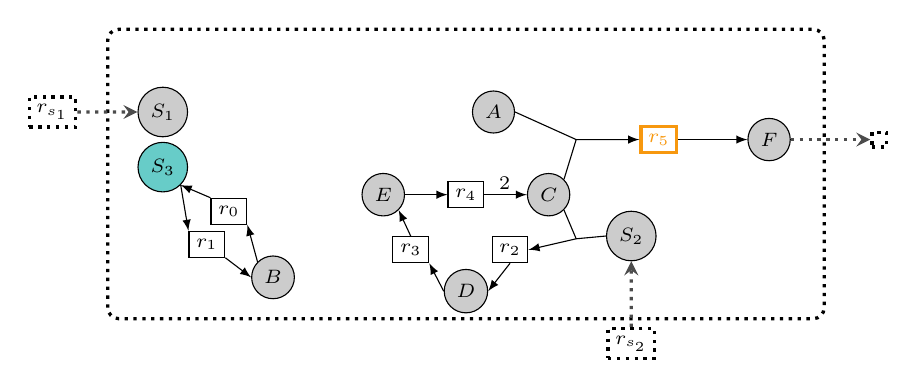
\begin{tikzpicture}[scale=0.7]\scriptsize
  \tikzstyle{metabolite}=[draw,circle,fill=white!80!black];
  \tikzstyle{repairmetabolite}=[draw,white!40!black, circle,fill=white!90!black,text=white!40!black,dashed];
  \tikzstyle{seed}=[draw,circle,fill=BlueGreen!70];%white!80!black
  \tikzstyle{target}=[draw,circle,fill=YellowOrange];%white!40!black
  \tikzstyle{reaction}=[draw,rectangle];
   \tikzstyle{export}=[draw,rectangle,dotted, very thick];
   \tikzstyle{exportrepair}=[draw,rectangle,dotted, very thick,white!80!black,text=white!70!black];
  \tikzstyle{repairreaction}=[draw,rectangle,white!40!black,text=white!40!black,dashed];
  \tikzstyle{initial}=[->,>=latex,thick];
  \tikzstyle{bdd}=[->,>=latex,thick];
  \tikzstyle{etiq}=[midway,fill=black!20,scale=0.5];
  \tikzstyle{stc}=[draw, rectangle, white, text=black]

  \node[stc] (stcr4C) at (6.2,6.7) {$2$};

  \draw [black,dotted, rounded corners, very thick] (-1,4.25) rectangle (12,9.5);
 % \node (system) [draw, rounded rectangle] at (0,0) {} (7cm,5cm);

  \node[seed] (S2) at (0,7) {$S_{3}$};
  \node[metabolite] (Sb2) at (8.5,5.75) {$S_{2}$};
  \node[metabolite] (S1) at (0,8) {$S_{1}$};

  \node[metabolite] (F) at (11,7.50) {$F$};

  \node[metabolite] (A) at (6,8) {$A$};
  \node[metabolite] (B) at (2,5.0) {$B$};
  \node[metabolite] (C) at (7,6.5) {$C$};
  \node[metabolite] (D) at (5.50,4.75) {$D$};
  \node[metabolite] (E) at (4,6.5) {$E$};
 % \node[repairmetabolite] (X) at (5,9) {$G$};

  \node[reaction] (R0) at (1.2,6.2) {$r_{0}$};
  \node[reaction] (R1) at (0.8,5.60) {$r_{1}$};
  \node[reaction] (R2) at (6.3,5.5) {$r_{2}$};
  \node[reaction] (R3) at (4.5,5.5) {$r_{3}$};
  \node[reaction] (R4) at (5.5,6.5) {$r_{4}$};
  \node[reaction, very thick,YellowOrange] (R5) at (9,7.50) {$r_{5}$}; %LimeGreen
  %\node[repairreaction] (R6) at (3,8) {$r_{6}$};
  %\node[repairreaction] (R7) at (2.3,6.9) {$r_{7}$};
  %\node[repairreaction] (R8) at (3,5.8) {$r_{8}$};
  %\node[repairreaction] (R9) at (8.5,8.5) {$r_{9}$};

  % R0 : S => B
  \draw[->,>=latex] (B.north west) -- (R0.south east);
  \draw[->,>=latex] (R0.north west) -- (S2.south east);

  % R1 : S <= B
  \draw[->,>=latex] (S2.south east) -- (R1.north west);
  \draw[->,>=latex] (R1.south east) -- (B.west);

  % R2 : Sb2+C => D
  \draw[->,>=latex] (Sb2.west) -- (7.5,5.70) -- (R2.east);
  \draw[] (C.south east) -- (7.5,5.70);
  \draw[->,>=latex] (R2.south) -- (D.east);

  % R3 : D => E
  \draw[->,>=latex] (D.west) -- (R3.south east);
  \draw[->,>=latex] (R3.north) -- (E.south east);

  % R4 : E => C
  \draw[->,>=latex] (E.east) -- (R4.west);
  \draw[->,>=latex] (R4.east) -- (C.west);

  % R5 : A+C => T
  \draw[->,>=latex] (A.east) -- (7.5,7.50) -- (R5.west);
  \draw[] (C.north east) -- (7.5,7.50);
  \draw[->,>=latex] (R5.east) -- (F.west);

  % R6 : S => A+X
 % \draw[->,>=latex,white!55!black,dashed] (S1.east) -- (R6.west);
  %\draw[->,>=latex,white!55!black,dashed] (R6.east) -- (4,8) -- (A.west);
  %\draw[->,>=latex,white!55!black,dashed] (4,8) -- (X.west);

  % R7 : S => E
 % \draw[->,>=latex,white!55!black,dashed] (S2.east) -- (R7.west);
  %\draw[->,>=latex,white!55!black,dashed] (R7.east) -- (E.north west);

  % R8 : B => E
 % \draw[->,>=latex,white!55!black,dashed] (B.north east) -- (R8.south west);
  %\draw[->,>=latex,white!55!black,dashed] (R8.east) -- (E.south);

  % R9 : X => F
 % \draw[->,>=latex,white!55!black,dashed] (X.east) -- (R9.north west);
  %\draw[->,>=latex,white!55!black,dashed] (R9.east) -- (F.north west);

  %export X
  %\node[exportrepair] (outX) at (6.5,10.30) {$r_{expX}$};
  %\draw[->,>=stealth,white!80!black,dotted, very thick] (X.north east) --  (outX.west);

  %export F
  \node[export] (outF) at (13,7.5) {\ExportReaction};
   \draw[->,>=stealth,white!30!black,dotted, very thick] (F.east) --  (outF.west);

  %import S2
   \node[export] (inS) at (-2,8) {$r_{s_1}$};
   \draw[->,>=stealth,white!30!black,dotted, very thick] (inS) --  (S1.west);

   %import Sb2
    \node[export] (inS2) at (8.5,3.8) {$r_{s_2}$};
    \draw[->,>=stealth,white!30!black,dotted, very thick] (inS2) --  (Sb2.south);

\end{tikzpicture}
%
%%% Local Variables:
%%% mode: latex
%%% TeX-master: "paper"
%%% End:

    \caption{Example of a metabolic network. Compounds and reactions are depicted by circles and rectangles respectively. Dashed reactions are reactions involving the boundary between the organism's metabolism and its environment. $r_5$ is the target reaction. $S_1$ and $S_2$ are boundary (and initiation) seeds. $S_3$ is assumed to be an initiation seed. Numbers on arrows describe the stoichiometry of reaction (default value is 1).}
    \label{gra:toy_d}
\end{figure}
% ----------------------------------------------------------------------
%
The network consists of 9 reactions, \SeedReaction, \SeedReactiont, \ExportReaction{} and $r_0$ to $r_5$, and 8 compounds, $A,\dots,F$, $S_1$, $S_2$ and $S_3$.
Here, $S=\{S_1,S_2,S_3\}$, $S_1$ and $S_2$ being the two boundary compounds of the network. Dashed rectangle describes the boundary of the system, outside of which is the environment of the organism.
%
Consider reaction
\(
r_4 : E\rightarrow 2C
\)
transforming one unit of $E$ into two units of $C$ (stoichiometric coefficients of 1 are omitted in the graphical representation; cf.~Fig.~\ref{gra:toy_d}).
%
We have
$\Reactants{r_4}=\{E\}$,
$\Products{r_4}=\{C\}$,
along with $\Stoichiometry{E}{r_4}=1 $
\ and $\Stoichiometry{r_4}{C}=2$.

In biology, several concepts have been introduced to model the activation of reaction fluxes in metabolic networks,
or to synthesize metabolic compounds.
%
To model this,
we introduce a function \ActivityFunction\ that given a metabolic network $G$ takes a set of seeds $S \subseteq M$ and returns a set of activated
reactions $\Activitytwo{G}{S} \subseteq R$.
%
%
% ----------------------------------------------------------------------
\begin{figure}[t]
  \centering
    %!TEX root = paper.tex
\usetikzlibrary{shapes.misc, positioning}
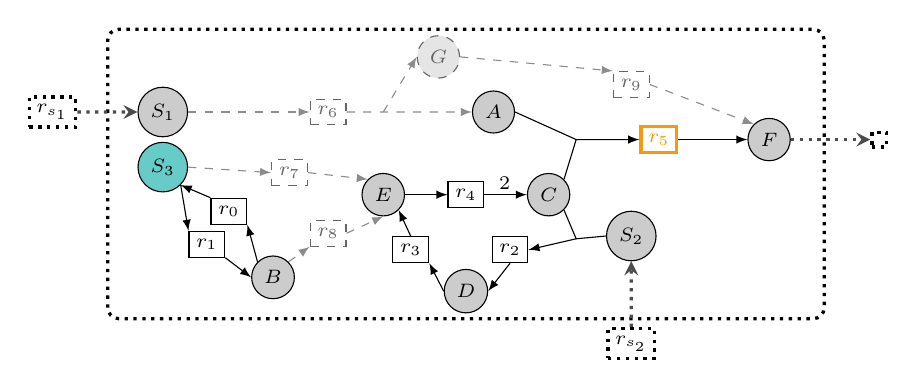
\begin{tikzpicture}[scale=0.7]\scriptsize
  \tikzstyle{metabolite}=[draw,circle,fill=white!80!black];
  \tikzstyle{repairmetabolite}=[draw,white!40!black, circle,fill=white!90!black,text=white!40!black,dashed];
  \tikzstyle{seed}=[draw,circle,fill=BlueGreen!70];%white!80!black
  \tikzstyle{target}=[draw,circle,fill=YellowOrange];%white!40!black
  \tikzstyle{reaction}=[draw,rectangle];
   \tikzstyle{export}=[draw,rectangle,dotted, very thick];
   \tikzstyle{exportrepair}=[draw,rectangle,dotted, very thick,white!80!black,text=white!70!black];
  \tikzstyle{repairreaction}=[draw,rectangle,white!40!black,text=white!40!black,dashed];
  \tikzstyle{initial}=[->,>=latex,thick];
  \tikzstyle{bdd}=[->,>=latex,thick];
  \tikzstyle{etiq}=[midway,fill=black!20,scale=0.5];
  \tikzstyle{stc}=[draw, rectangle, white, text=black]

  \node[stc] (stcr4C) at (6.2,6.7) {$2$};

  \draw [black,dotted, rounded corners, very thick] (-1,4.25) rectangle (12,9.5);
 % \node (system) [draw, rounded rectangle] at (0,0) {} (7cm,5cm);

  \node[seed] (S2) at (0,7) {$S_{3}$};
  \node[metabolite] (Sb2) at (8.5,5.75) {$S_{2}$};
  \node[metabolite] (S1) at (0,8) {$S_{1}$};

  \node[metabolite] (F) at (11,7.50) {$F$};

  \node[metabolite] (A) at (6,8) {$A$};
  \node[metabolite] (B) at (2,5.0) {$B$};
  \node[metabolite] (C) at (7,6.5) {$C$};
  \node[metabolite] (D) at (5.50,4.75) {$D$};
  \node[metabolite] (E) at (4,6.5) {$E$};
  \node[repairmetabolite] (X) at (5,9) {$G$};

  \node[reaction] (R0) at (1.2,6.2) {$r_{0}$};
  \node[reaction] (R1) at (0.8,5.60) {$r_{1}$};
  \node[reaction] (R2) at (6.3,5.5) {$r_{2}$};
  \node[reaction] (R3) at (4.5,5.5) {$r_{3}$};
  \node[reaction] (R4) at (5.5,6.5) {$r_{4}$};
  \node[reaction, very thick,YellowOrange] (R5) at (9,7.50) {$r_{5}$}; %LimeGreen
  \node[repairreaction] (R6) at (3,8) {$r_{6}$};
  \node[repairreaction] (R7) at (2.3,6.9) {$r_{7}$};
  \node[repairreaction] (R8) at (3,5.8) {$r_{8}$};
  \node[repairreaction] (R9) at (8.5,8.5) {$r_{9}$};

  % R0 : S => B
  \draw[->,>=latex] (B.north west) -- (R0.south east);
  \draw[->,>=latex] (R0.north west) -- (S2.south east);

  % R1 : S <= B
  \draw[->,>=latex] (S2.south east) -- (R1.north west);
  \draw[->,>=latex] (R1.south east) -- (B.west);

  % R2 : Sb2+C => D
  \draw[->,>=latex] (Sb2.west) -- (7.5,5.70) -- (R2.east);
  \draw[] (C.south east) -- (7.5,5.70);
  \draw[->,>=latex] (R2.south) -- (D.east);

  % R3 : D => E
  \draw[->,>=latex] (D.west) -- (R3.south east);
  \draw[->,>=latex] (R3.north) -- (E.south east);

  % R4 : E => C
  \draw[->,>=latex] (E.east) -- (R4.west);
  \draw[->,>=latex] (R4.east) -- (C.west);

  % R5 : A+C => T
  \draw[->,>=latex] (A.east) -- (7.5,7.50) -- (R5.west);
  \draw[] (C.north east) -- (7.5,7.50);
  \draw[->,>=latex] (R5.east) -- (F.west);

  % R6 : S => A+X
  \draw[->,>=latex,white!55!black,dashed] (S1.east) -- (R6.west);
  \draw[->,>=latex,white!55!black,dashed] (R6.east) -- (4,8) -- (A.west);
  \draw[->,>=latex,white!55!black,dashed] (4,8) -- (X.west);

  % R7 : S => E
  \draw[->,>=latex,white!55!black,dashed] (S2.east) -- (R7.west);
  \draw[->,>=latex,white!55!black,dashed] (R7.east) -- (E.north west);

  % R8 : B => E
  \draw[->,>=latex,white!55!black,dashed] (B.north east) -- (R8.south west);
  \draw[->,>=latex,white!55!black,dashed] (R8.east) -- (E.south);

  % R9 : X => F
  \draw[->,>=latex,white!55!black,dashed] (X.east) -- (R9.north west);
  \draw[->,>=latex,white!55!black,dashed] (R9.east) -- (F.north west);

  %export X
  %\node[exportrepair] (outX) at (6.5,10.30) {$r_{expX}$};
  %\draw[->,>=stealth,white!80!black,dotted, very thick] (X.north east) --  (outX.west);

  %export F
  \node[export] (outF) at (13,7.5) {\ExportReaction};
   \draw[->,>=stealth,white!30!black,dotted, very thick] (F.east) --  (outF.west);

   %import S2
    \node[export] (inS) at (-2,8) {$r_{s_1}$};
    \draw[->,>=stealth,white!30!black,dotted, very thick] (inS) --  (S1.west);

   %import Sb2
  \node[export] (inS2) at (8.5,3.8) {$r_{s_2}$};
  \draw[->,>=stealth,white!30!black,dotted, very thick] (inS2) --  (Sb2.south);

\end{tikzpicture}
%
%%% Local Variables:
%%% mode: latex
%%% TeX-master: "paper"
%%% End:

    \caption{Metabolic network completion problem. The purpose of its solving is to select the minimal number of reactions from a database (dashed shaded reactions) such that activation of target reaction $r_5$ is restored from boundary and/or initiation seeds. There are three formalisms for activation of target reaction: stoichiometric, topological and hybrid.}
    \label{gra:toy}
\end{figure}
% ----------------------------------------------------------------------
%
With it,
\emph{metabolic network completion} is about ensuring that a set of target reactions (reaction $r_5$ in~Fig.~\ref{gra:toy_d}) is activated from seed compounds in $S$
by possibly extending the metabolic network with reactions from a reference network (cf.\ shaded part in~Fig.~\ref{gra:toy}).

Formally, given
a metabolic network $G=(R\cup M,E,\StoichiometricFunction)$, % with bounds,
a set $S\subseteq M$ of seed compounds such that $\strseed(G) \subseteq S$,
a set $R_{T}\subseteq R$ of target reactions, and
a reference network $(R'\cup M',E',\StoichiometricFunction')$,
%
the \emph{metabolic network completion problem} is to find a set $R''\subseteq R'\setminus R$ of reactions of minimal size such that
\(
R_{T}\subseteq\Activitytwo{G''}{S}
\)
where%
\footnote{Since \StoichiometricFunction, $\StoichiometricFunction'$ have disjoint domains we view them as relations and compose them by union.}
\begin{align}
  \label{eq:completion:graph}
  G''&= ((R\cup R'')\cup (M\cup M''),E\cup E'',\StoichiometricFunction'')\ ,
  \\\label{eq:completion:metabolites}
  M''&=\{m\in M'\mid r\in R'', m\in\Reactants{r}\cup\Products{r}\}\ ,
  \\\label{eq:completion:edges}
  E''&=E'\cap((M''\times R'')\cup(R''\times M'')) , \text{ and}
  \\
  \StoichiometricFunction''&=\StoichiometricFunction\cup\StoichiometricFunction'
  \ .
\end{align}
%
We call $R''$ a \emph{completion} of $(R\cup M,E,\StoichiometricFunction)$ from $(R'\cup M',E',\StoichiometricFunction')$ wrt $S$ and $R_{T}$.
%
Our concept of activation allows different biological paradigms to be captured.
%
Accordingly,
different formulations of metabolic network completion can be characterized:
the stoichiometric, the relaxed stoichiometric, the topological, and the hybrid one.
We elaborate upon their formal characterizations in the following sections.

\subsection{Stoichiometric Metabolic Network Completion}\label{sec:stoichio} %\emph
%
The first activation semantics has been introduced in the context of Flux Balance Analysis
capturing reaction flux distributions of metabolic networks at steady state.
%
In this paradigm, each reaction $r$ is associated with a \emph{metabolic flux value},
expressed as a real variable $v_r$ confined by the minimum and maximum rates:
%
\begin{align} \label{eq:stoichiometric:bounds}
  & \MinFlux{r} \leq  v_r\leq \MaxFlux{r} \qquad\text{ for } r\in R.
\end{align}
%
Flux distributions are formalized in terms of a system of equations relying on the stoichiometric coefficients of reactions.
%
\review{Reaction stoichiometries are governed by the \emph{law of mass conservation} under a steady state assumption; in other words, the mass of the system remains constant over the reaction.
The input and output fluxes of reactions consuming and producing a metabolite are balanced.}
%
\begin{align}
\label{eq:stoichiometric:equation}
  & \textstyle
    \sum_{\substack{r\in R}}\Stoichiometry{r}{m}\cdot v_r
    +
    \sum_{\substack{r\in R}}-\Stoichiometry{m}{r}\cdot v_r
    =
    0
    \qquad \text{ for } m\in M.
\end{align}
%
Given a target reaction $r_T\in R_T$, a metabolic network $G=(R\cup M,E,\StoichiometricFunction)$ and a set of seeds $S$,
\emph{stoichiometric activation} is defined as follows:
\begin{align}%*
\label{eq:stoichiometric:activation}
  r_T \in \Activity{s}{G}{S} & \ \text{ iff } \ v_{r_T} >0 \text{ and }
                               \eqref{eq:stoichiometric:bounds} \text{ and } \eqref{eq:stoichiometric:equation}\text{ hold for }M\text{ and }R.
\end{align}%*
Note that the condition $v_{r_T} >0$ strengthens the flux condition for $r_T\in R$ in the second part.
More generally, observe that activated target reactions are not directly related to the network's seeds $S$.
However,
the activation of targets highly depends on the boundary compounds in $\strseed(G)$
for which \eqref{eq:stoichiometric:equation} \review{is always satisfied and thus initiates the fluxes.
Since boundary compounds are produced by at least one reaction without prerequisite,
an arbitrary amount might be produced.
Therefore, the incoming flux value always balances the sum of the flux values associated to outgoing edges.
Intuitively, boundary compounds are nutrients that are expected to be available in the system
for the consumption by the metabolic network,
thus initiating the reactions within.}
%
In our draft network $G$,
consisting of all \review{non-dashed} nodes and edges depicted in Fig.~\ref{gra:toy}
(viz.\ reactions \SeedReaction, \SeedReactiont, \ExportReaction{} and $r_0$ to $r_5$ and compounds $A,\dots,F$, $S_1$, $S_2$, and $S_3$ and $r_5$ the single target reaction)
and the reference network $G'$,
consisting of the shaded part of Fig~\ref{gra:toy},
(viz.\ reactions $r_6$ to $r_9$ and metabolite $G$)
a strict stoichiometry-based completion aims to obtain a solution with $r_5\in\Activity{s}{G''}{\{S_1,S_2,S_3\}}$ where $v_{r_5}$ is maximal.
%
This can be achieved by adding the completion $R''_1=\{r_{6},r_9\}$ (Fig.~\ref{gra:toy_ss}).
%
\review{The cycle made of compounds $E,C,D$ and the boundary seed $S_2$ is already balanced and notably self-activated.
Indeed, initiation of $D$ and $E$ producibility requires the producibility of $C$ (in addition to the presence of the boundary seed $S_2$) that itself depends on $D$ and $E$. Yet, according the flux conditions, that models steady state conditions, the cycle is activated.
Such self-activation of cyclic pathways is an inherent problem of purely stoichiometric approaches to network completion.
This is a drawback of the semantics because the effective activation of the cycle requires the additional (and unchecked) condition that at least one of the compounds was present as the initial state of the system. This could be the case provided there exist another way to enable the production of one or several components of the cycle (here an activable reaction producing $E$ for instance) \citep{Prigent2017}.}
%
The instance of Equation~\eqref{eq:stoichiometric:equation} controlling the reaction rates related to metabolite $C$ is
\(
2\cdot v_{r_4} - v_{r_2} - v_{r_5} = 0
\).


To solve metabolic network completion with flux-balance activated reactions,
Linear Programming can be used to maximize the flux rate $v_{r_T}$ provided that the linear constraints are satisfied.
%
Nonetheless, this problem turns out to be hard to solve in practice and existing approaches scale poorly to real-life applications (cf.~ \citep{Orth2010}).

This motivated the use of approximate methods.
%
The relaxed problem is obtained by weakening the mass-balance equation \eqref{eq:stoichiometric:equation} as follows:
%
\begin{align}
\label{eq:stoichiometric:equation:relaxed}
  &  \textstyle        \sum_{\substack{r\in R}} \Stoichiometry{r}{m}\cdot v_r
                       +
                       \sum_{\substack{r\in R}}-\Stoichiometry{m}{r}\cdot v_r
                       \geq
                       0
                       \qquad \text{ for } m\in M.
\end{align}
%
This lets us define the concept of \emph{relaxed stoichiometric activation}:
\begin{align}%*
\label{eq:stoichiometric:activation:relaxed}
  r_T \in \Activity{r}{G}{S} & \ \text{ iff } \ v_{r_T} >0 \text{ and }
                               \eqref{eq:stoichiometric:bounds} \text{ and } \eqref{eq:stoichiometric:equation:relaxed}\text{ hold for }M\text{ and }R.
\end{align}%*
The resulting problem can now be efficiently solved with Linear Programming~\citep{SatishKumar2007}.
%
Existing systems addressing strict stoichiometric network completion either
cannot guarantee optimal solutions~\citep{laten2014a} or
do not support a focus on specific target reactions~\citep{Thiele2014}.
Other approaches either partially relax the problem~\citep{Vitkin2012} or
solve the relaxed problem based on Equation~\eqref{eq:stoichiometric:equation:relaxed},
like the popular system \gapfill~\citep{SatishKumar2007}. Applied to the network of Fig.~\ref{gra:toy}, the minimal completion under the relaxed stoichiometric activation is $R''_1=\{r_{6}\}$  (Fig.~\ref{gra:toy_sr}) but does not carry flux because of the accumulation of metabolite $G$, allowed by Equation~\eqref{eq:stoichiometric:equation:relaxed}.
%
Note however that for strict steady-state modeling an \textit{a posteriori} verification of solutions is needed
to warrant the exact mass-balance equation~\eqref{eq:stoichiometric:equation}.


% ----------------------------------------------------------------------
\begin{figure}
    \captionsetup{width=0.45\textwidth}
    \centering
    \begin{minipage}[t]{.5\textwidth}
      \centering
      %!TEX root = paper.tex
\usetikzlibrary{shapes.misc, positioning}
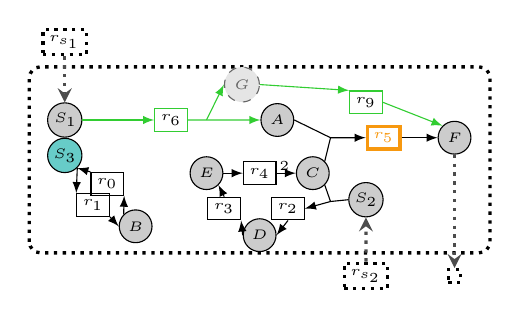
\begin{tikzpicture}[scale=0.45]\tiny
  \tikzstyle{metabolite}=[draw,circle,fill=white!80!black, text width=0.4cm, inner sep=0pt, align=center];
  \tikzstyle{repairmetabolite}=[draw,white!40!black, circle,fill=white!90!black,text=white!40!black,dashed];
  \tikzstyle{seed}=[draw,circle,fill=BlueGreen!70, text width=0.4cm, inner sep=0pt, align=center];%white!80!black
  \tikzstyle{target}=[draw,circle,fill=YellowOrange];%white!40!black
  \tikzstyle{reaction}=[draw,rectangle];
   \tikzstyle{export}=[draw,rectangle,dotted, very thick];
   \tikzstyle{exportrepair}=[draw,rectangle,dotted, very thick,white!80!black,text=white!70!black];
  \tikzstyle{repairreaction}=[draw,rectangle,white!40!black,text=white!40!black,dashed];
  \tikzstyle{solreaction}=[draw,rectangle,LimeGreen,text=black];
  \tikzstyle{initial}=[->,>=latex,thick];
  \tikzstyle{bdd}=[->,>=latex,thick];
  \tikzstyle{etiq}=[midway,fill=black!20,scale=0.5];
  \tikzstyle{stc}=[draw, rectangle, white, text=black]

  \node[stc] (stcr4C) at (6.2,6.7) {$2$};

  \draw [black,dotted, rounded corners, very thick] (-1,4.25) rectangle (12,9.5);
 % \node (system) [draw, rounded rectangle] at (0,0) {} (7cm,5cm);

  \node[seed] (S2) at (0,7) {$S_{3}$};
  \node[metabolite] (Sb2) at (8.5,5.75) {$S_{2}$};
  \node[metabolite] (S1) at (0,8) {$S_{1}$};

  \node[metabolite] (F) at (11,7.50) {$F$};

  \node[metabolite] (A) at (6,8) {$A$};
  \node[metabolite] (B) at (2,5.0) {$B$};
  \node[metabolite] (C) at (7,6.5) {$C$};
  \node[metabolite] (D) at (5.50,4.75) {$D$};
  \node[metabolite] (E) at (4,6.5) {$E$};
  \node[repairmetabolite] (X) at (5,9) {$G$};

  \node[reaction] (R0) at (1.2,6.2) {$r_{0}$};
  \node[reaction] (R1) at (0.8,5.60) {$r_{1}$};
  \node[reaction] (R2) at (6.3,5.5) {$r_{2}$};
  \node[reaction] (R3) at (4.5,5.5) {$r_{3}$};
  \node[reaction] (R4) at (5.5,6.5) {$r_{4}$};
  \node[reaction, very thick,YellowOrange] (R5) at (9,7.50) {$r_{5}$}; %LimeGreen
  \node[solreaction] (R6) at (3,8) {$r_{6}$};
  % \node[repairreaction] (R7) at (2.3,6.9) {$r_{7}$};
  % \node[repairreaction] (R8) at (3,5.8) {$r_{8}$};
  \node[solreaction] (R9) at (8.5,8.5) {$r_{9}$};

  % R0 : S => B
  \draw[->,>=latex] (B.north west) -- (R0.south east);
  \draw[->,>=latex] (R0.north west) -- (S2.south east);

  % R1 : S <= B
  \draw[->,>=latex] (S2.south east) -- (R1.north west);
  \draw[->,>=latex] (R1.south east) -- (B.west);

  % R2 : Sb2+C => D
  \draw[->,>=latex] (Sb2.west) -- (7.5,5.70) -- (R2.east);
  \draw[] (C.south east) -- (7.5,5.70);
  \draw[->,>=latex] (R2.south) -- (D.east);

  % R3 : D => E
  \draw[->,>=latex] (D.west) -- (R3.south east);
  \draw[->,>=latex] (R3.north) -- (E.south east);

  % R4 : E => C
  \draw[->,>=latex] (E.east) -- (R4.west);
  \draw[->,>=latex] (R4.east) -- (C.west);

  % R5 : A+C => T
  \draw[->,>=latex] (A.east) -- (7.5,7.50) -- (R5.west);
  \draw[] (C.north east) -- (7.5,7.50);
  \draw[->,>=latex] (R5.east) -- (F.west);

  % R6 : S => A+X
  \draw[->,>=latex,LimeGreen] (S1.east) -- (R6.west);
  \draw[->,>=latex,LimeGreen] (R6.east) -- (4,8) -- (A.west);
  \draw[->,>=latex,LimeGreen] (4,8) -- (X.west);

  % % R7 : S => E
  % \draw[->,>=latex,white!55!black,dashed] (S2.east) -- (R7.west);
  % \draw[->,>=latex,white!55!black,dashed] (R7.east) -- (E.north west);
  %
  % % R8 : B => E
  % \draw[->,>=latex,white!55!black,dashed] (B.north east) -- (R8.south west);
  % \draw[->,>=latex,white!55!black,dashed] (R8.east) -- (E.south);

  % R9 : X => F
  \draw[->,>=latex,LimeGreen] (X.east) -- (R9.north west);
  \draw[->,>=latex,LimeGreen] (R9.east) -- (F.north west);

  %export X
  %\node[exportrepair] (outX) at (6.5,10.30) {$r_{expX}$};
  %\draw[->,>=stealth,white!80!black,dotted, very thick] (X.north east) --  (outX.west);

  %export F
  \node[export] (outF) at (11,3.6) {\ExportReaction};
   \draw[->,>=stealth,white!30!black,dotted, very thick] (F.south) --  (outF.north);

  %import S2
   \node[export] (inS) at (0,10.2) {$r_{s_1}$};
   \draw[->,>=stealth,white!30!black,dotted, very thick] (inS.south) --  (S1.north);

   %import Sb2
  \node[export] (inS2) at (8.5,3.6) {$r_{s_2}$};
  \draw[->,>=stealth,white!30!black,dotted, very thick] (inS2) --  (Sb2.south);

\end{tikzpicture}
%
%%% Local Variables:
%%% mode: latex
%%% TeX-master: "paper"
%%% End:

      \caption{Solution to metabolic network completion under stoichiometric activation hypothesis in order to satisfy Equations~\eqref{eq:stoichiometric:bounds},~\eqref{eq:stoichiometric:equation} and ~\eqref{eq:stoichiometric:activation}. Within this network, there exists at least one flux distribution which activates $r_5$.}
      \label{gra:toy_ss}
    \end{minipage}%
    \begin{minipage}[t]{.5\textwidth}
      \centering
      %!TEX root = paper.tex
\usetikzlibrary{shapes.misc, positioning}
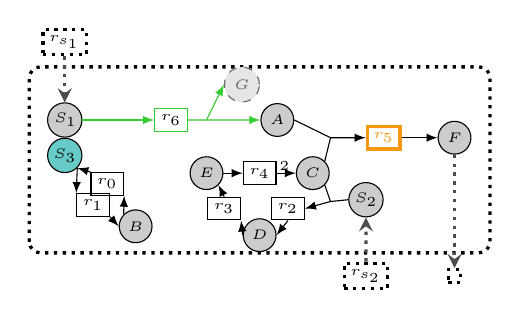
\begin{tikzpicture}[scale=0.45]\tiny
  \tikzstyle{metabolite}=[draw,circle,fill=white!80!black, text width=0.4cm, inner sep=0pt, align=center];
  \tikzstyle{repairmetabolite}=[draw,white!40!black, circle,fill=white!90!black,text=white!40!black,dashed];
  \tikzstyle{seed}=[draw,circle,fill=BlueGreen!70, text width=0.4cm, inner sep=0pt, align=center];%white!80!black
  \tikzstyle{target}=[draw,circle,fill=YellowOrange];%white!40!black
  \tikzstyle{reaction}=[draw,rectangle];
   \tikzstyle{export}=[draw,rectangle,dotted, very thick];
   \tikzstyle{exportrepair}=[draw,rectangle,dotted, very thick,white!80!black,text=white!70!black];
  \tikzstyle{repairreaction}=[draw,rectangle,white!40!black,text=white!40!black,dashed];
  \tikzstyle{solreaction}=[draw,rectangle,LimeGreen,text=black];
  \tikzstyle{initial}=[->,>=latex,thick];
  \tikzstyle{bdd}=[->,>=latex,thick];
  \tikzstyle{etiq}=[midway,fill=black!20,scale=0.5];
  \tikzstyle{stc}=[draw, rectangle, white, text=black]

  \node[stc] (stcr4C) at (6.2,6.7) {$2$};

  \draw [black,dotted, rounded corners, very thick] (-1,4.25) rectangle (12,9.5);
 % \node (system) [draw, rounded rectangle] at (0,0) {} (7cm,5cm);

  \node[seed] (S2) at (0,7) {$S_{3}$};
  \node[metabolite] (Sb2) at (8.5,5.75) {$S_{2}$};
  \node[metabolite] (S1) at (0,8) {$S_{1}$};

  \node[metabolite] (F) at (11,7.50) {$F$};

  \node[metabolite] (A) at (6,8) {$A$};
  \node[metabolite] (B) at (2,5.0) {$B$};
  \node[metabolite] (C) at (7,6.5) {$C$};
  \node[metabolite] (D) at (5.50,4.75) {$D$};
  \node[metabolite] (E) at (4,6.5) {$E$};
  \node[repairmetabolite] (X) at (5,9) {$G$};

  \node[reaction] (R0) at (1.2,6.2) {$r_{0}$};
  \node[reaction] (R1) at (0.8,5.60) {$r_{1}$};
  \node[reaction] (R2) at (6.3,5.5) {$r_{2}$};
  \node[reaction] (R3) at (4.5,5.5) {$r_{3}$};
  \node[reaction] (R4) at (5.5,6.5) {$r_{4}$};
  \node[reaction, very thick,YellowOrange] (R5) at (9,7.50) {$r_{5}$}; %LimeGreen
  \node[solreaction] (R6) at (3,8) {$r_{6}$};
  % \node[repairreaction] (R7) at (2.3,6.9) {$r_{7}$};
  % \node[repairreaction] (R8) at (3,5.8) {$r_{8}$};
  % \node[repairreaction] (R9) at (8.5,8.5) {$r_{9}$};

  % R0 : S => B
  \draw[->,>=latex] (B.north west) -- (R0.south east);
  \draw[->,>=latex] (R0.north west) -- (S2.south east);

  % R1 : S <= B
  \draw[->,>=latex] (S2.south east) -- (R1.north west);
  \draw[->,>=latex] (R1.south east) -- (B.west);

  % R2 : Sb2+C => D
  \draw[->,>=latex] (Sb2.west) -- (7.5,5.70) -- (R2.east);
  \draw[] (C.south east) -- (7.5,5.70);
  \draw[->,>=latex] (R2.south) -- (D.east);

  % R3 : D => E
  \draw[->,>=latex] (D.west) -- (R3.south east);
  \draw[->,>=latex] (R3.north) -- (E.south east);

  % R4 : E => C
  \draw[->,>=latex] (E.east) -- (R4.west);
  \draw[->,>=latex] (R4.east) -- (C.west);

  % R5 : A+C => T
  \draw[->,>=latex] (A.east) -- (7.5,7.50) -- (R5.west);
  \draw[] (C.north east) -- (7.5,7.50);
  \draw[->,>=latex] (R5.east) -- (F.west);

  % R6 : S => A+X
  \draw[->,>=latex,LimeGreen] (S1.east) -- (R6.west);
  \draw[->,>=latex,LimeGreen] (R6.east) -- (4,8) -- (A.west);
  \draw[->,>=latex,LimeGreen] (4,8) -- (X.west);

  % % R7 : S => E
  % \draw[->,>=latex,white!55!black,dashed] (S2.east) -- (R7.west);
  % \draw[->,>=latex,white!55!black,dashed] (R7.east) -- (E.north west);
  %
  % % R8 : B => E
  % \draw[->,>=latex,white!55!black,dashed] (B.north east) -- (R8.south west);
  % \draw[->,>=latex,white!55!black,dashed] (R8.east) -- (E.south);

  % % R9 : X => F
  % \draw[->,>=latex,green] (X.east) -- (R9.north west);
  % \draw[->,>=latex,green] (R9.east) -- (F.north west);

  %export X
  %\node[exportrepair] (outX) at (6.5,10.30) {$r_{expX}$};
  %\draw[->,>=stealth,white!80!black,dotted, very thick] (X.north east) --  (outX.west);

  %export F
  \node[export] (outF) at (11,3.6) {\ExportReaction};
   \draw[->,>=stealth,white!30!black,dotted, very thick] (F.south) --  (outF.north);

  %import S2
   \node[export] (inS) at (0,10.2) {$r_{s_1}$};
   \draw[->,>=stealth,white!30!black,dotted, very thick] (inS.south) --  (S1.north);

   %import Sb2
  \node[export] (inS2) at (8.5,3.6) {$r_{s_2}$};
  \draw[->,>=stealth,white!30!black,dotted, very thick] (inS2) --  (Sb2.south);

\end{tikzpicture}
%
%%% Local Variables:
%%% mode: latex
%%% TeX-master: "paper"
%%% End:

      \caption{Solution to metabolic network completion under relaxed stoichiometric activation hypothesis in order to satisfy Equations~\eqref{eq:stoichiometric:bounds},~\eqref{eq:stoichiometric:equation:relaxed} and ~\eqref{eq:stoichiometric:activation:relaxed}. Notice that within this completed network, there exist no flux distribution allowing the reaction $r_5$ to be activated.}
      \label{gra:toy_sr}
    \end{minipage}
\end{figure}
% ----------------------------------------------------------------------

\subsection{Topological Metabolic Network Completion}\label{sec:topo} %emph
%
A qualitative approach to metabolic network completion relies on the topology of networks for capturing the activation of reactions.
%
Given a metabolic network $G$, a reaction $r\in R$ is \emph{activated} from a set of seeds $S$ if all reactants in $\Reactants{r}$ are reachable from~$S$.
%
Moreover, a metabolite $m\in M$ is \emph{reachable} from $S$ if %
$m\in S$
or if
$m\in\Products{r}$ for some reaction $r\in R$ where all $m'\in\Reactants{r}$ are reachable from~$S$.
%
The \emph{scope} of $S$, written $\Sigma_G(S)$, is the closure of compounds reachable from~$S$.
%
In this setting, \emph{topological activation} of reactions from a set of seeds $S$ is defined as follows:
%
\begin{align}%*
  r_T \in \Activity{t}{G}{S} \ \text{ iff } \ \Reactants{r_T} \subseteq \Sigma_G(S).   \label{eq:topological:activation}
\end{align} %*
%
Note that this semantics avoids self-activated cycles by imposing an external entry sufficient to initiate all cycles ($S_3$ is not enough to activate the cycle as it does not activate one of its reaction on its own).
The resulting network completion problem can be expressed as a combinatorial optimization problem and effectively solved with ASP~\citep{schthi09a}.

For illustration, consider again the draft and reference networks $G$ and $G'$ in Fig.~\ref{gra:toy_d} and Fig.~\ref{gra:toy}.
%
We get $\Sigma_{G}(\{S_1,S_2,S_3\})=\{S_1,S_2,S_3,B\}$, indicating that target reaction $r_5$ is not activated from the seeds with the draft network
because $A$ and $C$, its reactants, are not reachable.
%
This changes once the network is completed.
%
Valid minimal completions are $R''_2=\{r_6,r_7\}$ (Fig.~\ref{gra:toy_st1}) and $R''_3=\{r_6,r_8\}$ (Fig.~\ref{gra:toy_st2}) because
\(
r_5\in\Activity{t}{G''_i}{\{S_1,S_2\}}\mbox{ since }\{A,C\}\subseteq\Sigma_{G''_i}(\{S_1,S_2\})
\)
for all extended networks $G''_i$ obtained from completions $R''_i$ of $G$ for $i\in\{2,3\}$.
%
% ----------------------------------------------------------------------
\begin{figure}
    \captionsetup{width=0.45\textwidth}
    \centering
    \begin{minipage}[t]{.5\textwidth}
      \centering
      %!TEX root = paper.tex
\usetikzlibrary{shapes.misc, positioning}
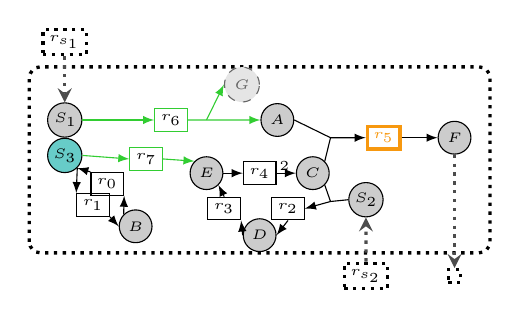
\begin{tikzpicture}[scale=0.45]\tiny
  \tikzstyle{metabolite}=[draw,circle,fill=white!80!black, text width=0.4cm, inner sep=0pt, align=center];
  \tikzstyle{repairmetabolite}=[draw,white!40!black, circle,fill=white!90!black,text=white!40!black,dashed];
  \tikzstyle{seed}=[draw,circle,fill=BlueGreen!70, text width=0.4cm, inner sep=0pt, align=center];%white!80!black
  \tikzstyle{target}=[draw,circle,fill=YellowOrange];%white!40!black
  \tikzstyle{reaction}=[draw,rectangle];
   \tikzstyle{export}=[draw,rectangle,dotted, very thick];
   \tikzstyle{exportrepair}=[draw,rectangle,dotted, very thick,white!80!black,text=white!70!black];
  \tikzstyle{repairreaction}=[draw,rectangle,white!40!black,text=white!40!black,dashed];
  \tikzstyle{solreaction}=[draw,rectangle,LimeGreen,text=black];
  \tikzstyle{initial}=[->,>=latex,thick];
  \tikzstyle{bdd}=[->,>=latex,thick];
  \tikzstyle{etiq}=[midway,fill=black!20,scale=0.5];
  \tikzstyle{stc}=[draw, rectangle, white, text=black]

  \node[stc] (stcr4C) at (6.2,6.7) {$2$};

  \draw [black,dotted, rounded corners, very thick] (-1,4.25) rectangle (12,9.5);
 % \node (system) [draw, rounded rectangle] at (0,0) {} (7cm,5cm);

  \node[seed] (S2) at (0,7) {$S_{3}$};
  \node[metabolite] (Sb2) at (8.5,5.75) {$S_{2}$};
  \node[metabolite] (S1) at (0,8) {$S_{1}$};

  \node[metabolite] (F) at (11,7.50) {$F$};

  \node[metabolite] (A) at (6,8) {$A$};
  \node[metabolite] (B) at (2,5.0) {$B$};
  \node[metabolite] (C) at (7,6.5) {$C$};
  \node[metabolite] (D) at (5.50,4.75) {$D$};
  \node[metabolite] (E) at (4,6.5) {$E$};
  \node[repairmetabolite] (X) at (5,9) {$G$};

  \node[reaction] (R0) at (1.2,6.2) {$r_{0}$};
  \node[reaction] (R1) at (0.8,5.60) {$r_{1}$};
  \node[reaction] (R2) at (6.3,5.5) {$r_{2}$};
  \node[reaction] (R3) at (4.5,5.5) {$r_{3}$};
  \node[reaction] (R4) at (5.5,6.5) {$r_{4}$};
  \node[reaction, very thick,YellowOrange] (R5) at (9,7.50) {$r_{5}$}; %LimeGreen
  \node[solreaction] (R6) at (3,8) {$r_{6}$};
  \node[solreaction] (R7) at (2.3,6.9) {$r_{7}$};
  % \node[repairreaction] (R8) at (3,5.8) {$r_{8}$};
  % \node[repairreaction] (R9) at (8.5,8.5) {$r_{9}$};

  % R0 : S => B
  \draw[->,>=latex] (B.north west) -- (R0.south east);
  \draw[->,>=latex] (R0.north west) -- (S2.south east);

  % R1 : S <= B
  \draw[->,>=latex] (S2.south east) -- (R1.north west);
  \draw[->,>=latex] (R1.south east) -- (B.west);

  % R2 : Sb2+C => D
  \draw[->,>=latex] (Sb2.west) -- (7.5,5.70) -- (R2.east);
  \draw[] (C.south east) -- (7.5,5.70);
  \draw[->,>=latex] (R2.south) -- (D.east);

  % R3 : D => E
  \draw[->,>=latex] (D.west) -- (R3.south east);
  \draw[->,>=latex] (R3.north) -- (E.south east);

  % R4 : E => C
  \draw[->,>=latex] (E.east) -- (R4.west);
  \draw[->,>=latex] (R4.east) -- (C.west);

  % R5 : A+C => T
  \draw[->,>=latex] (A.east) -- (7.5,7.50) -- (R5.west);
  \draw[] (C.north east) -- (7.5,7.50);
  \draw[->,>=latex] (R5.east) -- (F.west);

  % R6 : S => A+X
  \draw[->,>=latex,LimeGreen] (S1.east) -- (R6.west);
  \draw[->,>=latex,LimeGreen] (R6.east) -- (4,8) -- (A.west);
  \draw[->,>=latex,LimeGreen] (4,8) -- (X.west);

  % R7 : S => E
  \draw[->,>=latex,LimeGreen] (S2.east) -- (R7.west);
  \draw[->,>=latex,LimeGreen] (R7.east) -- (E.north west);
  %
  % % R8 : B => E
  % \draw[->,>=latex,white!55!black,dashed] (B.north east) -- (R8.south west);
  % \draw[->,>=latex,white!55!black,dashed] (R8.east) -- (E.south);

  % % R9 : X => F
  % \draw[->,>=latex,green] (X.east) -- (R9.north west);
  % \draw[->,>=latex,green] (R9.east) -- (F.north west);

  %export X
  %\node[exportrepair] (outX) at (6.5,10.30) {$r_{expX}$};
  %\draw[->,>=stealth,white!80!black,dotted, very thick] (X.north east) --  (outX.west);

  %export F
  \node[export] (outF) at (11,3.6) {\ExportReaction};
   \draw[->,>=stealth,white!30!black,dotted, very thick] (F.south) --  (outF.north);

  %import S2
   \node[export] (inS) at (0,10.2) {$r_{s_1}$};
   \draw[->,>=stealth,white!30!black,dotted, very thick] (inS.south) --  (S1.north);

   %import Sb2
  \node[export] (inS2) at (8.5,3.6) {$r_{s_2}$};
  \draw[->,>=stealth,white!30!black,dotted, very thick] (inS2) --  (Sb2.south);

\end{tikzpicture}
%
%%% Local Variables:
%%% mode: latex
%%% TeX-master: "paper"
%%% End:

      \caption{First solution to metabolic network completion under topological activation hypothesis satisfying Equation~\eqref{eq:topological:activation}. The production of C cannot be explained by a self-activated cycle and requires an external source of compounds via $S_3$ and reaction $r_7$.}
      \label{gra:toy_st1}
    \end{minipage}%
    \begin{minipage}[t]{.5\textwidth}
      \centering
      %!TEX root = paper.tex
\usetikzlibrary{shapes.misc, positioning}
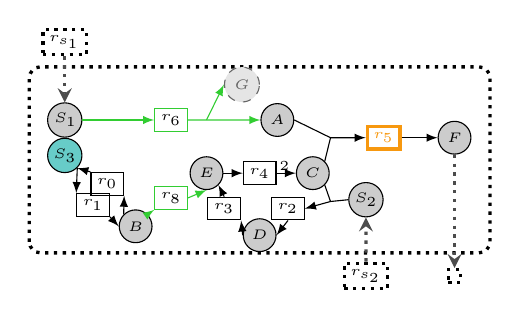
\begin{tikzpicture}[scale=0.45]\tiny
  \tikzstyle{metabolite}=[draw,circle,fill=white!80!black, text width=0.4cm, inner sep=0pt, align=center];
  \tikzstyle{repairmetabolite}=[draw,white!40!black, circle,fill=white!90!black,text=white!40!black,dashed];
  \tikzstyle{seed}=[draw,circle,fill=BlueGreen!70, text width=0.4cm, inner sep=0pt, align=center];%white!80!black
  \tikzstyle{target}=[draw,circle,fill=YellowOrange];%white!40!black
  \tikzstyle{reaction}=[draw,rectangle];
   \tikzstyle{export}=[draw,rectangle,dotted, very thick];
   \tikzstyle{exportrepair}=[draw,rectangle,dotted, very thick,white!80!black,text=white!70!black];
  \tikzstyle{repairreaction}=[draw,rectangle,white!40!black,text=white!40!black,dashed];
  \tikzstyle{solreaction}=[draw,rectangle,LimeGreen,text=black];
  \tikzstyle{initial}=[->,>=latex,thick];
  \tikzstyle{bdd}=[->,>=latex,thick];
  \tikzstyle{etiq}=[midway,fill=black!20,scale=0.5];
  \tikzstyle{stc}=[draw, rectangle, white, text=black]

  \node[stc] (stcr4C) at (6.2,6.7) {$2$};

  \draw [black,dotted, rounded corners, very thick] (-1,4.25) rectangle (12,9.5);
 % \node (system) [draw, rounded rectangle] at (0,0) {} (7cm,5cm);

  \node[seed] (S2) at (0,7) {$S_{3}$};
  \node[metabolite] (Sb2) at (8.5,5.75) {$S_{2}$};
  \node[metabolite] (S1) at (0,8) {$S_{1}$};

  \node[metabolite] (F) at (11,7.50) {$F$};

  \node[metabolite] (A) at (6,8) {$A$};
  \node[metabolite] (B) at (2,5.0) {$B$};
  \node[metabolite] (C) at (7,6.5) {$C$};
  \node[metabolite] (D) at (5.50,4.75) {$D$};
  \node[metabolite] (E) at (4,6.5) {$E$};
  \node[repairmetabolite] (X) at (5,9) {$G$};

  \node[reaction] (R0) at (1.2,6.2) {$r_{0}$};
  \node[reaction] (R1) at (0.8,5.60) {$r_{1}$};
  \node[reaction] (R2) at (6.3,5.5) {$r_{2}$};
  \node[reaction] (R3) at (4.5,5.5) {$r_{3}$};
  \node[reaction] (R4) at (5.5,6.5) {$r_{4}$};
  \node[reaction, very thick,YellowOrange] (R5) at (9,7.50) {$r_{5}$}; %LimeGreen
  \node[solreaction] (R6) at (3,8) {$r_{6}$};
  % \node[solreaction] (R7) at (2.3,6.9) {$r_{7}$};
  \node[solreaction] (R8) at (3,5.8) {$r_{8}$};
  % \node[repairreaction] (R9) at (8.5,8.5) {$r_{9}$};

  % R0 : S => B
  \draw[->,>=latex] (B.north west) -- (R0.south east);
  \draw[->,>=latex] (R0.north west) -- (S2.south east);

  % R1 : S <= B
  \draw[->,>=latex] (S2.south east) -- (R1.north west);
  \draw[->,>=latex] (R1.south east) -- (B.west);

  % R2 : Sb2+C => D
  \draw[->,>=latex] (Sb2.west) -- (7.5,5.70) -- (R2.east);
  \draw[] (C.south east) -- (7.5,5.70);
  \draw[->,>=latex] (R2.south) -- (D.east);

  % R3 : D => E
  \draw[->,>=latex] (D.west) -- (R3.south east);
  \draw[->,>=latex] (R3.north) -- (E.south east);

  % R4 : E => C
  \draw[->,>=latex] (E.east) -- (R4.west);
  \draw[->,>=latex] (R4.east) -- (C.west);

  % R5 : A+C => T
  \draw[->,>=latex] (A.east) -- (7.5,7.50) -- (R5.west);
  \draw[] (C.north east) -- (7.5,7.50);
  \draw[->,>=latex] (R5.east) -- (F.west);

  % R6 : S => A+X
  \draw[->,>=latex,LimeGreen] (S1.east) -- (R6.west);
  \draw[->,>=latex,LimeGreen] (R6.east) -- (4,8) -- (A.west);
  \draw[->,>=latex,LimeGreen] (4,8) -- (X.west);

  % % R7 : S => E
  % \draw[->,>=latex,white!55!black,dashed] (S2.east) -- (R7.west);
  % \draw[->,>=latex,white!55!black,dashed] (R7.east) -- (E.north west);

  % R8 : B => E
  \draw[->,>=latex,LimeGreen] (B.north east) -- (R8.south west);
  \draw[->,>=latex,LimeGreen] (R8.east) -- (E.south);

  % % R9 : X => F
  % \draw[->,>=latex,green] (X.east) -- (R9.north west);
  % \draw[->,>=latex,green] (R9.east) -- (F.north west);

  %export X
  %\node[exportrepair] (outX) at (6.5,10.30) {$r_{expX}$};
  %\draw[->,>=stealth,white!80!black,dotted, very thick] (X.north east) --  (outX.west);

  %export F
  \node[export] (outF) at (11,3.6) {\ExportReaction};
   \draw[->,>=stealth,white!30!black,dotted, very thick] (F.south) --  (outF.north);

  %import S2
   \node[export] (inS) at (0,10.2) {$r_{s_1}$};
   \draw[->,>=stealth,white!30!black,dotted, very thick] (inS.south) --  (S1.north);

   %import Sb2
  \node[export] (inS2) at (8.5,3.6) {$r_{s_2}$};
  \draw[->,>=stealth,white!30!black,dotted, very thick] (inS2) --  (Sb2.south);

\end{tikzpicture}
%
%%% Local Variables:
%%% mode: latex
%%% TeX-master: "paper"
%%% End:

      \caption{Second solution to metabolic network completion under topological activation hypothesis satisfying Equation~\eqref{eq:topological:activation}.}
      \label{gra:toy_st2}
    \end{minipage}
\end{figure}
% ----------------------------------------------------------------------

Relevant elements from the reference network are given in dashed gray.

\subsection{Hybrid Metabolic Network Completion}\label{sec:hybrid} %emph
%
The idea of hybrid metabolic network completion is to combine the two previous activation semantics:
the topological one accounts for a well-founded initiation of the system from the seeds
and the stoichiometric one warrants its mass-balance.
%
We thus aim at network completions that are both topologically functional and flux balanced
(without suffering from self-activated cycles).
%
More precisely,
a reaction $r_T\in R_T$ is \emph{hybridly activated} from a set $S$ of seeds in a network $G$,
if both criteria apply:
%
\begin{align}%*
\label{eq:hybrid:activation}
%\[
r_T \in \Activity{h}{G}{S} \ \text{ iff } \ r_T \in \Activity{s}{G}{S}\text{ and }r_T \in \Activity{t}{G}{S}.
%\]
\end{align}%*

Applying this to our example in Fig.~\ref{gra:toy},
we get the (minimal) hybrid solutions $R''_4=\{r_6,r_7,r_{9}\}$ (Fig.~\ref{gra:toy_sh1}) and $R''_5=\{r_6,r_8,r_{9}\}$ (Fig.~\ref{gra:toy_sh2}).
Both (topologically) initiate paths of reactions from the seeds to the target,
ie.\ $r_5\in\Activity{t}{G''_i}{\{S_1,S_2,S_3\}}\mbox{ since }\{A,C\}\subseteq\Sigma_{G''_i}(\{S_1,S_2,S_3\})$
for both extended networks $G''_i$ obtained from completions $R''_i$ of $G$ for $i\in\{4,5\}$.
Both solutions are as well stoichiometrically valid and balance the amount of every metabolite,
hence we also have $r_5\in\Activity{s}{G''_i}{\{S_1,S_2,S_3\}}$.

% ----------------------------------------------------------------------
\begin{figure}
    \captionsetup{width=0.45\textwidth}
    \centering
    \begin{minipage}[t]{.50\textwidth}
      \centering
      %!TEX root = paper.tex
\usetikzlibrary{shapes.misc, positioning}
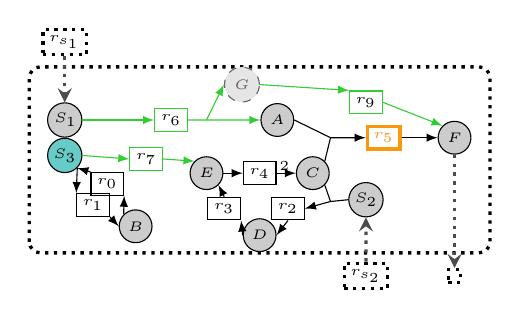
\begin{tikzpicture}[scale=0.45]\tiny
  \tikzstyle{metabolite}=[draw,circle,fill=white!80!black, text width=0.4cm, inner sep=0pt, align=center];
  \tikzstyle{repairmetabolite}=[draw,white!40!black, circle,fill=white!90!black,text=white!40!black,dashed];
  \tikzstyle{seed}=[draw,circle,fill=BlueGreen!70, text width=0.4cm, inner sep=0pt, align=center];%white!80!black
  \tikzstyle{target}=[draw,circle,fill=YellowOrange];%white!40!black
  \tikzstyle{reaction}=[draw,rectangle];
   \tikzstyle{export}=[draw,rectangle,dotted, very thick];
   \tikzstyle{exportrepair}=[draw,rectangle,dotted, very thick,white!80!black,text=white!70!black];
  \tikzstyle{repairreaction}=[draw,rectangle,white!40!black,text=white!40!black,dashed];
  \tikzstyle{solreaction}=[draw,rectangle,LimeGreen,text=black];
  \tikzstyle{initial}=[->,>=latex,thick];
  \tikzstyle{bdd}=[->,>=latex,thick];
  \tikzstyle{etiq}=[midway,fill=black!20,scale=0.5];
  \tikzstyle{stc}=[draw, rectangle, white, text=black]

  \node[stc] (stcr4C) at (6.2,6.7) {$2$};

  \draw [black,dotted, rounded corners, very thick] (-1,4.25) rectangle (12,9.5);
 % \node (system) [draw, rounded rectangle] at (0,0) {} (7cm,5cm);

  \node[seed] (S2) at (0,7) {$S_{3}$};
  \node[metabolite] (Sb2) at (8.5,5.75) {$S_{2}$};
  \node[metabolite] (S1) at (0,8) {$S_{1}$};

  \node[metabolite] (F) at (11,7.50) {$F$};

  \node[metabolite] (A) at (6,8) {$A$};
  \node[metabolite] (B) at (2,5.0) {$B$};
  \node[metabolite] (C) at (7,6.5) {$C$};
  \node[metabolite] (D) at (5.50,4.75) {$D$};
  \node[metabolite] (E) at (4,6.5) {$E$};
  \node[repairmetabolite] (X) at (5,9) {$G$};

  \node[reaction] (R0) at (1.2,6.2) {$r_{0}$};
  \node[reaction] (R1) at (0.8,5.60) {$r_{1}$};
  \node[reaction] (R2) at (6.3,5.5) {$r_{2}$};
  \node[reaction] (R3) at (4.5,5.5) {$r_{3}$};
  \node[reaction] (R4) at (5.5,6.5) {$r_{4}$};
  \node[reaction, very thick,YellowOrange] (R5) at (9,7.50) {$r_{5}$}; %LimeGreen
  \node[solreaction] (R6) at (3,8) {$r_{6}$};
  \node[solreaction] (R7) at (2.3,6.9) {$r_{7}$};
  % \node[repairreaction] (R8) at (3,5.8) {$r_{8}$};
  \node[solreaction] (R9) at (8.5,8.5) {$r_{9}$};

  % R0 : S => B
  \draw[->,>=latex] (B.north west) -- (R0.south east);
  \draw[->,>=latex] (R0.north west) -- (S2.south east);

  % R1 : S <= B
  \draw[->,>=latex] (S2.south east) -- (R1.north west);
  \draw[->,>=latex] (R1.south east) -- (B.west);

  % R2 : Sb2+C => D
  \draw[->,>=latex] (Sb2.west) -- (7.5,5.70) -- (R2.east);
  \draw[] (C.south east) -- (7.5,5.70);
  \draw[->,>=latex] (R2.south) -- (D.east);

  % R3 : D => E
  \draw[->,>=latex] (D.west) -- (R3.south east);
  \draw[->,>=latex] (R3.north) -- (E.south east);

  % R4 : E => C
  \draw[->,>=latex] (E.east) -- (R4.west);
  \draw[->,>=latex] (R4.east) -- (C.west);

  % R5 : A+C => T
  \draw[->,>=latex] (A.east) -- (7.5,7.50) -- (R5.west);
  \draw[] (C.north east) -- (7.5,7.50);
  \draw[->,>=latex] (R5.east) -- (F.west);

  % R6 : S => A+X
  \draw[->,>=latex,LimeGreen] (S1.east) -- (R6.west);
  \draw[->,>=latex,LimeGreen] (R6.east) -- (4,8) -- (A.west);
  \draw[->,>=latex,LimeGreen] (4,8) -- (X.west);

  % R7 : S => E
  \draw[->,>=latex,LimeGreen] (S2.east) -- (R7.west);
  \draw[->,>=latex,LimeGreen] (R7.east) -- (E.north west);
  %
  % % R8 : B => E
  % \draw[->,>=latex,white!55!black,dashed] (B.north east) -- (R8.south west);
  % \draw[->,>=latex,white!55!black,dashed] (R8.east) -- (E.south);

  % R9 : X => F
  \draw[->,>=latex,LimeGreen] (X.east) -- (R9.north west);
  \draw[->,>=latex,LimeGreen] (R9.east) -- (F.north west);

  %export X
  %\node[exportrepair] (outX) at (6.5,10.30) {$r_{expX}$};
  %\draw[->,>=stealth,white!80!black,dotted, very thick] (X.north east) --  (outX.west);

  %export F
  \node[export] (outF) at (11,3.6) {\ExportReaction};
   \draw[->,>=stealth,white!30!black,dotted, very thick] (F.south) --  (outF.north);

  %import S2
   \node[export] (inS) at (0,10.2) {$r_{s_1}$};
   \draw[->,>=stealth,white!30!black,dotted, very thick] (inS.south) --  (S1.north);

   %import Sb2
  \node[export] (inS2) at (8.5,3.6) {$r_{s_2}$};
  \draw[->,>=stealth,white!30!black,dotted, very thick] (inS2) --  (Sb2.south);

\end{tikzpicture}
%
%%% Local Variables:
%%% mode: latex
%%% TeX-master: "paper"
%%% End:

      \caption{First solution to metabolic network completion under hybrid activation hypothesis satisfying Equation~\eqref{eq:hybrid:activation} (that is Equations~\eqref{eq:stoichiometric:bounds},~\eqref{eq:stoichiometric:equation}, ~\eqref{eq:stoichiometric:activation} and ~\eqref{eq:topological:activation}).}
      \label{gra:toy_sh1}
    \end{minipage}%
    \begin{minipage}[t]{.50\textwidth}
      \centering
      %!TEX root = paper.tex
\usetikzlibrary{shapes.misc, positioning}
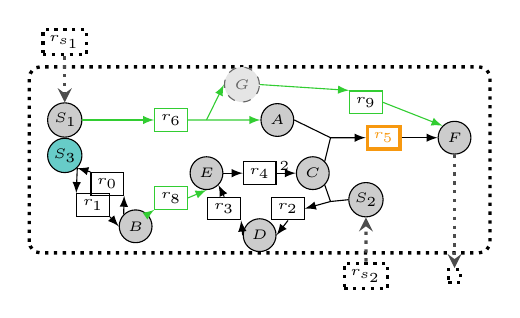
\begin{tikzpicture}[scale=0.45]\tiny
  \tikzstyle{metabolite}=[draw,circle,fill=white!80!black, text width=0.4cm, inner sep=0pt, align=center];
  \tikzstyle{repairmetabolite}=[draw,white!40!black, circle,fill=white!90!black,text=white!40!black,dashed];
  \tikzstyle{seed}=[draw,circle,fill=BlueGreen!70, text width=0.4cm, inner sep=0pt, align=center];%white!80!black
  \tikzstyle{target}=[draw,circle,fill=YellowOrange];%white!40!black
  \tikzstyle{reaction}=[draw,rectangle];
   \tikzstyle{export}=[draw,rectangle,dotted, very thick];
   \tikzstyle{exportrepair}=[draw,rectangle,dotted, very thick,white!80!black,text=white!70!black];
  \tikzstyle{repairreaction}=[draw,rectangle,white!40!black,text=white!40!black,dashed];
  \tikzstyle{solreaction}=[draw,rectangle,LimeGreen,text=black];
  \tikzstyle{initial}=[->,>=latex,thick];
  \tikzstyle{bdd}=[->,>=latex,thick];
  \tikzstyle{etiq}=[midway,fill=black!20,scale=0.5];
  \tikzstyle{stc}=[draw, rectangle, white, text=black]

  \node[stc] (stcr4C) at (6.2,6.7) {$2$};

  \draw [black,dotted, rounded corners, very thick] (-1,4.25) rectangle (12,9.5);
 % \node (system) [draw, rounded rectangle] at (0,0) {} (7cm,5cm);

  \node[seed] (S2) at (0,7) {$S_{3}$};
  \node[metabolite] (Sb2) at (8.5,5.75) {$S_{2}$};
  \node[metabolite] (S1) at (0,8) {$S_{1}$};

  \node[metabolite] (F) at (11,7.50) {$F$};

  \node[metabolite] (A) at (6,8) {$A$};
  \node[metabolite] (B) at (2,5.0) {$B$};
  \node[metabolite] (C) at (7,6.5) {$C$};
  \node[metabolite] (D) at (5.50,4.75) {$D$};
  \node[metabolite] (E) at (4,6.5) {$E$};
  \node[repairmetabolite] (X) at (5,9) {$G$};

  \node[reaction] (R0) at (1.2,6.2) {$r_{0}$};
  \node[reaction] (R1) at (0.8,5.60) {$r_{1}$};
  \node[reaction] (R2) at (6.3,5.5) {$r_{2}$};
  \node[reaction] (R3) at (4.5,5.5) {$r_{3}$};
  \node[reaction] (R4) at (5.5,6.5) {$r_{4}$};
  \node[reaction, very thick,YellowOrange] (R5) at (9,7.50) {$r_{5}$}; %LimeGreen
  \node[solreaction] (R6) at (3,8) {$r_{6}$};
  % \node[solreaction] (R7) at (2.3,6.9) {$r_{7}$};
  \node[solreaction] (R8) at (3,5.8) {$r_{8}$};
  \node[solreaction] (R9) at (8.5,8.5) {$r_{9}$};

  % R0 : S => B
  \draw[->,>=latex] (B.north west) -- (R0.south east);
  \draw[->,>=latex] (R0.north west) -- (S2.south east);

  % R1 : S <= B
  \draw[->,>=latex] (S2.south east) -- (R1.north west);
  \draw[->,>=latex] (R1.south east) -- (B.west);

  % R2 : Sb2+C => D
  \draw[->,>=latex] (Sb2.west) -- (7.5,5.70) -- (R2.east);
  \draw[] (C.south east) -- (7.5,5.70);
  \draw[->,>=latex] (R2.south) -- (D.east);

  % R3 : D => E
  \draw[->,>=latex] (D.west) -- (R3.south east);
  \draw[->,>=latex] (R3.north) -- (E.south east);

  % R4 : E => C
  \draw[->,>=latex] (E.east) -- (R4.west);
  \draw[->,>=latex] (R4.east) -- (C.west);

  % R5 : A+C => T
  \draw[->,>=latex] (A.east) -- (7.5,7.50) -- (R5.west);
  \draw[] (C.north east) -- (7.5,7.50);
  \draw[->,>=latex] (R5.east) -- (F.west);

  % R6 : S => A+X
  \draw[->,>=latex,LimeGreen] (S1.east) -- (R6.west);
  \draw[->,>=latex,LimeGreen] (R6.east) -- (4,8) -- (A.west);
  \draw[->,>=latex,LimeGreen] (4,8) -- (X.west);

  % % R7 : S => E
  % \draw[->,>=latex,white!55!black,dashed] (S2.east) -- (R7.west);
  % \draw[->,>=latex,white!55!black,dashed] (R7.east) -- (E.north west);

  % R8 : B => E
  \draw[->,>=latex,LimeGreen] (B.north east) -- (R8.south west);
  \draw[->,>=latex,LimeGreen] (R8.east) -- (E.south);

  % R9 : X => F
  \draw[->,>=latex,LimeGreen] (X.east) -- (R9.north west);
  \draw[->,>=latex,LimeGreen] (R9.east) -- (F.north west);

  %export X
  %\node[exportrepair] (outX) at (6.5,10.30) {$r_{expX}$};
  %\draw[->,>=stealth,white!80!black,dotted, very thick] (X.north east) --  (outX.west);

  %export F
  \node[export] (outF) at (11,3.6) {\ExportReaction};
   \draw[->,>=stealth,white!30!black,dotted, very thick] (F.south) --  (outF.north);

  %import S2
   \node[export] (inS) at (0,10.2) {$r_{s_1}$};
   \draw[->,>=stealth,white!30!black,dotted, very thick] (inS.south) --  (S1.north);

   %import Sb2
  \node[export] (inS2) at (8.5,3.6) {$r_{s_2}$};
  \draw[->,>=stealth,white!30!black,dotted, very thick] (inS2) --  (Sb2.south);

\end{tikzpicture}
%
%%% Local Variables:
%%% mode: latex
%%% TeX-master: "paper"
%%% End:

      \caption{Second solution to metabolic network completion under hybrid activation hypothesis satisfying Equation~\eqref{eq:hybrid:activation} (that is Equations~\eqref{eq:stoichiometric:bounds},~\eqref{eq:stoichiometric:equation}, ~\eqref{eq:stoichiometric:activation} and ~\eqref{eq:topological:activation}).}
      \label{gra:toy_sh2}
    \end{minipage}
\end{figure}
% ----------------------------------------------------------------------

\subsection{Union of Metabolic Network Completions}\label{sec:union} %emph
As depicted in the toy examples for the topological (Fig.~\ref{gra:toy_st1} and Fig.~\ref{gra:toy_st2}) and hybrid (Fig.~\ref{gra:toy_sh1} and
Fig.~\ref{gra:toy_sh2}) activation, several minimal solutions to one metabolic network completion problem may exist.
There might be dozens of minimal completions, depending on the degradation of the original draft network,
hence leading to difficulties for biologists and bioinformaticians to discriminate the individual results.
One solution to facilitate this curation task is to provide, in addition to the enumeration of solutions, their union.
This has been done previously for the topological completion \citep{Prigent2017}.

% \begin{itemize}
%  \item Since we are able to verify activation for the union of networks,
%        offers us to analyze the quality of approximation methods, like topological and relaxed stoichiometric completion.
%  \item Thus, the idea to union solutions of approximation methods is,
%        to get a may non-minimal set of reactions, which is interesting to may satisfy activation.
% \end{itemize}
Notably, the concept of ``union of solutions" is particularly relevant from the biological perspective since it provides in a single view all possible reactions that could be inserted in a solution to the network completion problem.
%
Additionally, verifying the union according to the desired (stoichiometric and hybrid) activation semantics,
offers a way to analyze the quality of approximation methods (topological and relaxed-stoichiometric ones).
If individual solutions contradict a definition of activation that the union satisfies, it suggests that the family of reactions contained in the union, although possibly non-minimal, may be of interest.
Thus providing merit to the approximation method and their results.

Importantly, we notice that the operation of performing the union of solutions is stable with the concept of activation, although it can contradict the minimality of the size of completion.
Indeed, the union of solutions to the topological network completion problem is itself a (non-minimal) solution to the topological completion problem.
Similarly, the union of minimal stoichiometric solutions always displays the stoichiometric activation of the target reaction(s).
In fact, adding an arbitrary set of reactions to a metabolic network still maintains stoichiometric activation,
since flux distribution for the newly added reactions may be set to zero.
Consequently, the union of minimal hybrid solutions always displays the hybrid activation in the target reaction(s).
%

The following theorems (Theorems ~\ref{th:topo}, ~\ref{th:flux} and ~\ref{th:hybr}) are a formalization of the stability of the union of solutions with respect to the three concepts of activation.


The union $G=G_1\cup G_2$ of two metabolic networks $G_1=(R_1\cup M_1,E_1,\StoichiometricFunction_1)$
and $G_2=(R_2\cup M_2,E_2,\StoichiometricFunction_2)$ is defined by
\begin{align}
G &= (R\cup M, E, \StoichiometricFunction), \label{eq:graph.union1}\\
R &= R_1\cup R_2, \label{eq:graph.union2}\\
M &= M_1\cup M_2, \label{eq:graph.union3}\\
E &= E_1\cup E_2, \label{eq:graph.union4}\\
\StoichiometricFunction &= \StoichiometricFunction_1\cup \StoichiometricFunction_2. \label{eq:graph.union5}
\end{align}

\begin{theorem}\label{th:topo}
Let $G_1$ and $G_2$ be metabolic networks.
If $R_T\subseteq\Activity{t}{G_1}{S}$, then $R_T\subseteq\Activity{t}{G_1\cup G_2}{S}$.
\end{theorem}

\begin{proof}
The proof is given by monotonicity of the union and the monotonicity of the closure.
Thus it can never be case that having more reactions disables reachability.
More formal,
$R_T\subseteq\Activity{t}{G_1}{S}$ holds iff
$\Reactants{r_T}\subseteq\Sigma_{G_1}(S)$.
Furthermore, we have
$\Sigma_{G_1}(S)\subseteq \Sigma_{G_1\cup G_2}(S)$
by the definition of the closure.
This implies
$\Reactants{r_T}\subseteq\Sigma_{G_1\cup G_2}(S)$.
Finally, we have
$R_T\subseteq\Activity{t}{G_1\cup G_2}{S}$.
\end{proof}


\begin{theorem}\label{th:flux}
Let $G_1$ and $G_2$ be metabolic networks.
If $R_T\subseteq\Activity{s}{G_1}{S}$, then $R_T\subseteq\Activity{s}{G_1\cup G_2}{S}$.
\end{theorem}

\begin{proof}
First, we define following bijective functions
\begin{align*}
f:&R_1 \rightarrow \{1,\dots,l\}\subseteq\mathbb{N}, \\
& r \mapsto f(r)=i \\
g:&M_1 \rightarrow \{1,\dots,k\}\subseteq\mathbb{N}, \\
& m \mapsto g(m)=j \\
f':&R_1\cup R_2 \rightarrow \{1,\dots,l'\}\subseteq\mathbb{N}, \\
& r \mapsto f'(r)=
    \begin{cases}
    f(r) &, \text{ if $f(r)$ is defined} \\
    i    &, \text{ otherwise}
    \end{cases} \\
g'&:M_1\cup M_2 \rightarrow \{1,\dots,k'\}\subseteq\mathbb{N} \\
& m \mapsto g'(m)=
    \begin{cases}
    g(m) &, \text{ if $g(m)$ is defined} \\
    j    &, \text{ otherwise}
    \end{cases}
\end{align*}
for $k=|M_1|$, $l=|R_1|$, $k'=|M_1\cup M_2|$ and $l'=|R_1\cup R_2|$ regarding $G_1$ and $G_1\cup G_2$, respectively.
Now, we rewrite the system of (\ref{eq:stoichiometric:equation}) regarding $G_1$ as a matrix equation $Av=0$ of form
\begin{align*}
\begin{pmatrix}
a_{11} & \dots & a_{1l} \\
\vdots & \ddots & \vdots \\
a_{k1} & \dots & a_{kl}
\end{pmatrix}
\begin{pmatrix}
v_1 \\
\vdots  \\
v_l
\end{pmatrix}
=
\begin{pmatrix}
0 \\
\vdots \\
0
\end{pmatrix}\label{eq:matrix}
\end{align*}
where $A$ is a $k\times l$ matrix with coefficients
\begin{align*}
%h: & M_1\times R_1 \rightarrow \mathbb{R} \\
%& (m,r) \mapsto h(m,r)=
a_{g(m)f(r)}=
    \begin{cases}
    \StoichiometricFunction_1(r,m)  &, (r,m)\in E_1 \\
    -\StoichiometricFunction_1(m,r) &, (m,r)\in E_1 \\
    0       &, \text{ otherwise}
    \end{cases}
\end{align*}
and $v$ consists of variables $v_{f(r)}$ for $r\in R_1$.
By $L=\{v\mid Av=0\}$ we denote the set of solutions induced by $Av=0$.

Furthermore, we represent the system of linear equations of (\ref{eq:stoichiometric:equation}) regarding $G_1\cup G_2$ as a matrix equation $A'v'=0$ of form
\begin{align*}
\begin{pmatrix}
a_{11} & \dots & a_{1l} & a_{1l+1} & \dots & a_{1l'} \\
\vdots & \ddots& \vdots & \vdots   & \ddots& \vdots \\
a_{k1} & \dots & a_{kl} & a_{kl+1} & \dots & a_{kl'} \\
0      & \dots & 0      & a_{k+1l+1} & \dots & a_{k+1l'} \\
\vdots & \ddots& \vdots & \vdots   & \ddots& \vdots \\
0      & \dots & 0      & a_{k'l+1}& \dots & a_{k'l'}
\end{pmatrix}
\begin{pmatrix}
v_1 \\
\vdots  \\
v_l \\
v_{l+1} \\
\vdots \\
v_{l'}
\end{pmatrix}
=
\begin{pmatrix}
0 \\
\vdots \\
0
\end{pmatrix}%\label{eq:matrix2}
\end{align*}
where $A'$ is a $k'\times l'$ matrix with coefficients
\begin{align*}
% h': & (M_1\cup M_2)\times(R_1\cup R_2) \rightarrow \mathbb{R} \\
%& (m,r) \mapsto h'(m,r)=
a_{g'(m)f'(r)}=
    \begin{cases}
    \StoichiometricFunction(r,m)  &, (r,m)\in E_1\cup E_2 \\
    -\StoichiometricFunction(m,r) &, (m,r)\in E_1\cup E_2 \\
    0       &, \text{ otherwise}
    \end{cases}
\end{align*}
where $\StoichiometricFunction=\StoichiometricFunction_1\cup \StoichiometricFunction_2$
and $v'$ consists of variables $v_{f'(r)}$ of (\ref{eq:stoichiometric:equation}) for $r\in R_1\cup R_2$.
Note that $A'$ can always be written in this form, since switching columns and rows will not change solutions.
By $L'=\{v'\mid A'v'=0\}$ we denote the set of solutions induced by $A'v'=0$.

Since $A'v'=0$ is homogeneous, $L\subseteq L'$ holds by extending $L$ with zeros for $v_{f'(r)}$ with $r\in R_2\setminus R_1$.
Thus $\{v\mid v\in L, \forall r_T\in R_T, v_{f(r_T)}>0\}
\subseteq\{v\mid v\in L', \forall r_T\in R_T, v_{f'(r_T)}>0\}$
by extending the first set with zeros for $v_{f'(r)}$ with $r\in R_2\setminus R_1$.
From $R_T\subseteq\Activity{s}{G_1}{S}$, we know that the homogeneous system of linear equations from
(\ref{eq:stoichiometric:equation}) regarding $G_1$ is non-trivial satisfiable,
which finally implies that $R_T\subseteq\Activity{s}{G_1\cup G_2}{S}$.
\end{proof}


\begin{theorem}\label{th:hybr}
Let $G_1$ and $G_2$ be metabolic networks.
If $R_T\subseteq\Activity{h}{G_1}{S}$, then $R_T\subseteq\Activity{h}{G_1\cup G_2}{S}$.
\end{theorem}

\begin{proof}
Follows directly by the definition of hybrid activation together with Theorem~\ref{th:topo} and Theorem~\ref{th:flux}.
More formal,
$R_T\subseteq\Activity{h}{G_1}{S}$
holds iff
$R_T\subseteq\Activity{t}{G_1}{S}$ and $R_T\subseteq\Activity{s}{G_1}{S}$.
From Theorem~\ref{th:topo} and $R_T\subseteq\Activity{t}{G_1}{S}$ follows
$R_T\subseteq\Activity{t}{G_1\cup G_2}{S}$.
Analogously, from Theorem~\ref{th:flux} and $R_T\subseteq\Activity{s}{G_1}{S}$ follows
$R_T\subseteq\Activity{s}{G_1\cup G_2}{S}$.
Finally, this implies
$R_T\subseteq\Activity{h}{G_1\cup G_2}{S}$.
\end{proof}



In particular, studying the union in case of topological modeling can pinpoint interesting cases.
Individual solutions satisfying the topological activation can additionally satisfy the stoichiometric and thus the hybrid activation semantics.
A union including such a solution will also adhere to the hybrid standard.
In some cases, the union of solutions will display the stoichiometric activation whereas the individual solutions only satisfy the topological activation.
Fig.~\ref{gra:union_nf_f1} to Fig.~\ref{gra:union_nf_f} display an example of topological metabolic network completions that do not satisfy stoichiometric (and hybrid) activation whereas their union does.
Fig.~\ref{gra:union_nf_nf1} to Fig.~\ref{gra:union_nf_nf} provide an example of minimal topological completions that do not satisfy stoichiometric (and hybrid) activation and for which the union does not satisfy it either.
%
%Both observations induce that in general we cannot derive anything about activation of reactions for an unionized graph if both of the previous graphs do not satisfy activation of these reactions as well.


Both observations induce that in general we cannot derive anything about activation of reactions in a graph resulting from the union of two or more graphs.
And similarly, we cannot infer about the activation of reactions in subgraphs arbitrarily derived from a graph in which these reactions are activated.


% ----------------------------------------------------------------------
\begin{figure}
    \captionsetup{width=0.3\textwidth}
    \centering
    \begin{minipage}[t]{.32\textwidth}
      % \documentclass{article}
% \usepackage[dvipsnames]{xcolor}
% \usepackage{tikz}
% \usepackage{xcolor,colortbl}
% 
% \begin{document}
% 
% \newcommand{\gringo}{\textit{gringo}}
\newcommand{\clasp}{\textit{clasp}}
\newcommand{\clingo}{\textit{clingo}}
\newcommand{\asprin}{\textit{asprin}}
\newcommand{\asap}{\textit{teaspoon}}
\newcommand{\piclasp}{\textit{piclasp}}

\newcommand{\code}[1]{\lstinline[basicstyle=\ttfamily]{#1}}

\newcommand{\lw}[1]{\smash{\lower1.ex\hbox{#1}}}
\newcommand{\llw}[1]{\smash{\lower3.ex\hbox{#1}}}

%\newcommand{\dataCL}[5]{%
%  \code{#1} & #3 & #5 & #4
%}
%\newcommand{\dataCS}[5]{%
%  #3 & #5 & #4
%}

\newenvironment{tableC}{%
  \scriptsize
  \tabcolsep = 0.6mm
  \begin{tabular}[t]{l|rlr|rlr|rlr|rlr|rlr}\hline
    \multicolumn{1}{l|}{\llw{Instance}} &
    \multicolumn{3}{c|}{UD1} &
    \multicolumn{3}{c|}{UD2} &
    \multicolumn{3}{c|}{UD3} &
    \multicolumn{3}{c|}{UD4} &
    \multicolumn{3}{c}{UD5} \\
    & 
    \multicolumn{1}{c}{Best} & & \multicolumn{1}{c|}{\emph{tea-}} & 
    \multicolumn{1}{c}{Best} & & \multicolumn{1}{c|}{\emph{tea-}} & 
    \multicolumn{1}{c}{Best} & & \multicolumn{1}{c|}{\emph{tea-}} & 
    \multicolumn{1}{c}{Best} & & \multicolumn{1}{c|}{\emph{tea-}} & 
    \multicolumn{1}{c}{Best} & & \multicolumn{1}{c}{\emph{tea-}} \\
    & 
    known & & \emph{spoon} & 
    known & & \emph{spoon} & 
    known & & \emph{spoon} & 
    known & & \emph{spoon} & 
    known & & \emph{spoon} \\
    \hline
  }{%
    \hline
  \end{tabular}
}

\newenvironment{tableB}{%
  \scriptsize
  \tabcolsep = 0.7mm
%  \begin{tabular}[t]{|l|c|r|l|l|l|}\hline
  \begin{tabular}[t]{lcrlll}\hline
    Instance &
    Formulation &
    Time (sec.)\\
    \hline
  }{%
    \hline
  \end{tabular}
}
\newenvironment{tableL}{%
  \scriptsize
  \tabcolsep = 0.7mm
  \begin{tabular}[t]{l|rrrrrrrr|r}\hline
    \lw{Instance} &
    \lw{Time (sec.)} &
    \multicolumn{6}{c}{The best utility vector} &
    The sum of  &
    The best of basic\\
    &
    &
    $(S_1,$ & $S_4,$ & $S_2,$ & $S_7,$ & $S_6,$ & $S_3)$ &
    utility vector &
    and optimized \\
    \hline
  }{%
    \hline
  \end{tabular}
}

%%% Local Variables:
%%% mode: latex
%%% TeX-master: "paper"
%%% End:


% \begin{figure}[t]
%   \centering

    \usetikzlibrary{shapes.misc, positioning}
    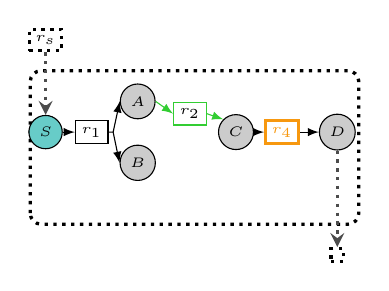
\begin{tikzpicture}[scale=0.39]\tiny
      \tikzstyle{metabolite}=[draw,circle,fill=white!80!black];
      \tikzstyle{repairmetabolite}=[draw,white!40!black, circle,fill=white!90!black,text=white!40!black,dashed];
      \tikzstyle{seed}=[draw,circle,fill=BlueGreen!70];%white!80!black
      \tikzstyle{target}=[draw,circle,fill=YellowOrange];%white!40!black
      \tikzstyle{reaction}=[draw,rectangle];
       \tikzstyle{export}=[draw,rectangle,dotted, very thick];
       \tikzstyle{exportrepair}=[draw,rectangle,dotted, very thick,white!80!black,text=white!70!black];
      \tikzstyle{repairreaction}=[draw,rectangle,white!40!black,text=white!40!black,dashed];
      \tikzstyle{solreaction}=[draw,rectangle,LimeGreen,text=black];
      \tikzstyle{initial}=[->,>=latex,thick];
      \tikzstyle{bdd}=[->,>=latex,thick];
      \tikzstyle{etiq}=[midway,fill=black!20,scale=0.5];
      \tikzstyle{stc}=[draw, rectangle, white, text=black]


      \draw [black,dotted, rounded corners, very thick] (-0.5,4) rectangle (10.2,9);
     % \node (system) [draw, rounded rectangle] at (0,0) {} (7cm,5cm);

      \node[seed] (S) at (0,7) {$S$};
      \node[metabolite] (A) at (3,8) {$A$};
      \node[metabolite] (B) at (3,6) {$B$};
      \node[metabolite] (C) at (6.2,7) {$C$};
      \node[metabolite] (D) at (9.5,7) {$D$};

      \node[reaction] (R1) at (1.5,7) {$r_{1}$};
      \node[reaction, very thick,YellowOrange] (R4) at (7.7,7) {$r_{4}$}; %LimeGreen
      \node[solreaction] (R2) at (4.7,7.6) {$r_{2}$};
      %\node[solreaction] (R3) at (4.7,6.4) {$r_{3}$};

      % R1 : S => A + B
      \draw[->,>=latex] (S.east) -- (R1.west);
      \draw[->,>=latex] (R1.east) -- (2.2,7) -- (A.west);
      \draw[->,>=latex] (2.2,7)  -- (B.west);

      % R2 : A => C
      \draw[->,>=latex,LimeGreen] (A.east) -- (R2.west);
      \draw[->,>=latex,LimeGreen] (R2.east) -- (C.north west);

      % R3 : B => C
      %\draw[->,>=latex,LimeGreen] (B.east) -- (R3.west);
      %\draw[->,>=latex,LimeGreen] (R3.east) -- (C.south west);

      % R4 : C => D
      \draw[->,>=latex] (C.east) -- (R4.west);
      \draw[->,>=latex] (R4.east) -- (D.west);

      %export G
      \node[export] (outD) at (9.5,3) {\ExportReaction};
      \draw[->,>=stealth,white!30!black,dotted, very thick] (D.south) --  (outD.north);

      %import S2
      \node[export] (inS) at (0,10) {$r_{s}$};
      \draw[->,>=stealth,white!30!black,dotted, very thick] (inS) --  (S.north);

  \end{tikzpicture}
% \end{figure}

% \end{document}

      \caption{Topological completion $R_1=\{r_2\}$ satisfies $r_4\in\Activity{t}{G_1}{\{S\}}$, but carries no flux, due to accumulation of compound $B$ that contradicts Eq.~\ref{eq:stoichiometric:equation}.\label{gra:union_nf_f1}}
    \end{minipage}
    \begin{minipage}[t]{.32\textwidth}
      % \documentclass{article}
% \usepackage[dvipsnames]{xcolor}
% \usepackage{tikz}
% \usepackage{xcolor,colortbl}
% 
% \begin{document}
% 
% \newcommand{\gringo}{\textit{gringo}}
\newcommand{\clasp}{\textit{clasp}}
\newcommand{\clingo}{\textit{clingo}}
\newcommand{\asprin}{\textit{asprin}}
\newcommand{\asap}{\textit{teaspoon}}
\newcommand{\piclasp}{\textit{piclasp}}

\newcommand{\code}[1]{\lstinline[basicstyle=\ttfamily]{#1}}

\newcommand{\lw}[1]{\smash{\lower1.ex\hbox{#1}}}
\newcommand{\llw}[1]{\smash{\lower3.ex\hbox{#1}}}

%\newcommand{\dataCL}[5]{%
%  \code{#1} & #3 & #5 & #4
%}
%\newcommand{\dataCS}[5]{%
%  #3 & #5 & #4
%}

\newenvironment{tableC}{%
  \scriptsize
  \tabcolsep = 0.6mm
  \begin{tabular}[t]{l|rlr|rlr|rlr|rlr|rlr}\hline
    \multicolumn{1}{l|}{\llw{Instance}} &
    \multicolumn{3}{c|}{UD1} &
    \multicolumn{3}{c|}{UD2} &
    \multicolumn{3}{c|}{UD3} &
    \multicolumn{3}{c|}{UD4} &
    \multicolumn{3}{c}{UD5} \\
    & 
    \multicolumn{1}{c}{Best} & & \multicolumn{1}{c|}{\emph{tea-}} & 
    \multicolumn{1}{c}{Best} & & \multicolumn{1}{c|}{\emph{tea-}} & 
    \multicolumn{1}{c}{Best} & & \multicolumn{1}{c|}{\emph{tea-}} & 
    \multicolumn{1}{c}{Best} & & \multicolumn{1}{c|}{\emph{tea-}} & 
    \multicolumn{1}{c}{Best} & & \multicolumn{1}{c}{\emph{tea-}} \\
    & 
    known & & \emph{spoon} & 
    known & & \emph{spoon} & 
    known & & \emph{spoon} & 
    known & & \emph{spoon} & 
    known & & \emph{spoon} \\
    \hline
  }{%
    \hline
  \end{tabular}
}

\newenvironment{tableB}{%
  \scriptsize
  \tabcolsep = 0.7mm
%  \begin{tabular}[t]{|l|c|r|l|l|l|}\hline
  \begin{tabular}[t]{lcrlll}\hline
    Instance &
    Formulation &
    Time (sec.)\\
    \hline
  }{%
    \hline
  \end{tabular}
}
\newenvironment{tableL}{%
  \scriptsize
  \tabcolsep = 0.7mm
  \begin{tabular}[t]{l|rrrrrrrr|r}\hline
    \lw{Instance} &
    \lw{Time (sec.)} &
    \multicolumn{6}{c}{The best utility vector} &
    The sum of  &
    The best of basic\\
    &
    &
    $(S_1,$ & $S_4,$ & $S_2,$ & $S_7,$ & $S_6,$ & $S_3)$ &
    utility vector &
    and optimized \\
    \hline
  }{%
    \hline
  \end{tabular}
}

%%% Local Variables:
%%% mode: latex
%%% TeX-master: "paper"
%%% End:


% \begin{figure}[t]
%   \centering

    \usetikzlibrary{shapes.misc, positioning}
    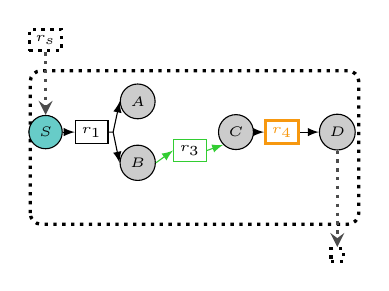
\begin{tikzpicture}[scale=0.39]\tiny
      \tikzstyle{metabolite}=[draw,circle,fill=white!80!black];
      \tikzstyle{repairmetabolite}=[draw,white!40!black, circle,fill=white!90!black,text=white!40!black,dashed];
      \tikzstyle{seed}=[draw,circle,fill=BlueGreen!70];%white!80!black
      \tikzstyle{target}=[draw,circle,fill=YellowOrange];%white!40!black
      \tikzstyle{reaction}=[draw,rectangle];
       \tikzstyle{export}=[draw,rectangle,dotted, very thick];
       \tikzstyle{exportrepair}=[draw,rectangle,dotted, very thick,white!80!black,text=white!70!black];
      \tikzstyle{repairreaction}=[draw,rectangle,white!40!black,text=white!40!black,dashed];
      \tikzstyle{solreaction}=[draw,rectangle,LimeGreen,text=black];
      \tikzstyle{initial}=[->,>=latex,thick];
      \tikzstyle{bdd}=[->,>=latex,thick];
      \tikzstyle{etiq}=[midway,fill=black!20,scale=0.5];
      \tikzstyle{stc}=[draw, rectangle, white, text=black]


      \draw [black,dotted, rounded corners, very thick] (-0.5,4) rectangle (10.2,9);
     % \node (system) [draw, rounded rectangle] at (0,0) {} (7cm,5cm);

      \node[seed] (S) at (0,7) {$S$};
      \node[metabolite] (A) at (3,8) {$A$};
      \node[metabolite] (B) at (3,6) {$B$};
      \node[metabolite] (C) at (6.2,7) {$C$};
      \node[metabolite] (D) at (9.5,7) {$D$};

      \node[reaction] (R1) at (1.5,7) {$r_{1}$};
      \node[reaction, very thick,YellowOrange] (R4) at (7.7,7) {$r_{4}$}; %LimeGreen
      %\node[solreaction] (R2) at (4.7,7.6) {$r_{2}$};
      \node[solreaction] (R3) at (4.7,6.4) {$r_{3}$};

      % R1 : S => A + B
      \draw[->,>=latex] (S.east) -- (R1.west);
      \draw[->,>=latex] (R1.east) -- (2.2,7) -- (A.west);
      \draw[->,>=latex] (2.2,7)  -- (B.west);

      % R2 : A => C
      %\draw[->,>=latex,LimeGreen] (A.east) -- (R2.west);
      %\draw[->,>=latex,LimeGreen] (R2.east) -- (C.north west);

      % R3 : B => C
      \draw[->,>=latex,LimeGreen] (B.east) -- (R3.west);
      \draw[->,>=latex,LimeGreen] (R3.east) -- (C.south west);

      % R4 : C => D
      \draw[->,>=latex] (C.east) -- (R4.west);
      \draw[->,>=latex] (R4.east) -- (D.west);

      %export G
      \node[export] (outD) at (9.5,3) {\ExportReaction};
      \draw[->,>=stealth,white!30!black,dotted, very thick] (D.south) --  (outD.north);

      %import S2
      \node[export] (inS) at (0,10) {$r_{s}$};
      \draw[->,>=stealth,white!30!black,dotted, very thick] (inS) --  (S.north);

  \end{tikzpicture}
% \end{figure}

% \end{document}

      \caption{Topological completion $R_2=\{r_3\}$ satisfies $r_4\in\Activity{t}{G_2}{\{S\}}$ and carries no flux as well, due to accumulation of compound $A$ that contradicts Eq.~\ref{eq:stoichiometric:equation}.\label{gra:union_nf_f2}}
    \end{minipage}
    \begin{minipage}[t]{.32\textwidth}
      % \documentclass{article}
% \usepackage[dvipsnames]{xcolor}
% \usepackage{tikz}
% \usepackage{xcolor,colortbl}
% 
% \begin{document}
% 
% \newcommand{\gringo}{\textit{gringo}}
\newcommand{\clasp}{\textit{clasp}}
\newcommand{\clingo}{\textit{clingo}}
\newcommand{\asprin}{\textit{asprin}}
\newcommand{\asap}{\textit{teaspoon}}
\newcommand{\piclasp}{\textit{piclasp}}

\newcommand{\code}[1]{\lstinline[basicstyle=\ttfamily]{#1}}

\newcommand{\lw}[1]{\smash{\lower1.ex\hbox{#1}}}
\newcommand{\llw}[1]{\smash{\lower3.ex\hbox{#1}}}

%\newcommand{\dataCL}[5]{%
%  \code{#1} & #3 & #5 & #4
%}
%\newcommand{\dataCS}[5]{%
%  #3 & #5 & #4
%}

\newenvironment{tableC}{%
  \scriptsize
  \tabcolsep = 0.6mm
  \begin{tabular}[t]{l|rlr|rlr|rlr|rlr|rlr}\hline
    \multicolumn{1}{l|}{\llw{Instance}} &
    \multicolumn{3}{c|}{UD1} &
    \multicolumn{3}{c|}{UD2} &
    \multicolumn{3}{c|}{UD3} &
    \multicolumn{3}{c|}{UD4} &
    \multicolumn{3}{c}{UD5} \\
    & 
    \multicolumn{1}{c}{Best} & & \multicolumn{1}{c|}{\emph{tea-}} & 
    \multicolumn{1}{c}{Best} & & \multicolumn{1}{c|}{\emph{tea-}} & 
    \multicolumn{1}{c}{Best} & & \multicolumn{1}{c|}{\emph{tea-}} & 
    \multicolumn{1}{c}{Best} & & \multicolumn{1}{c|}{\emph{tea-}} & 
    \multicolumn{1}{c}{Best} & & \multicolumn{1}{c}{\emph{tea-}} \\
    & 
    known & & \emph{spoon} & 
    known & & \emph{spoon} & 
    known & & \emph{spoon} & 
    known & & \emph{spoon} & 
    known & & \emph{spoon} \\
    \hline
  }{%
    \hline
  \end{tabular}
}

\newenvironment{tableB}{%
  \scriptsize
  \tabcolsep = 0.7mm
%  \begin{tabular}[t]{|l|c|r|l|l|l|}\hline
  \begin{tabular}[t]{lcrlll}\hline
    Instance &
    Formulation &
    Time (sec.)\\
    \hline
  }{%
    \hline
  \end{tabular}
}
\newenvironment{tableL}{%
  \scriptsize
  \tabcolsep = 0.7mm
  \begin{tabular}[t]{l|rrrrrrrr|r}\hline
    \lw{Instance} &
    \lw{Time (sec.)} &
    \multicolumn{6}{c}{The best utility vector} &
    The sum of  &
    The best of basic\\
    &
    &
    $(S_1,$ & $S_4,$ & $S_2,$ & $S_7,$ & $S_6,$ & $S_3)$ &
    utility vector &
    and optimized \\
    \hline
  }{%
    \hline
  \end{tabular}
}

%%% Local Variables:
%%% mode: latex
%%% TeX-master: "paper"
%%% End:


% \begin{figure}[t]
%   \centering

    \usetikzlibrary{shapes.misc, positioning}
    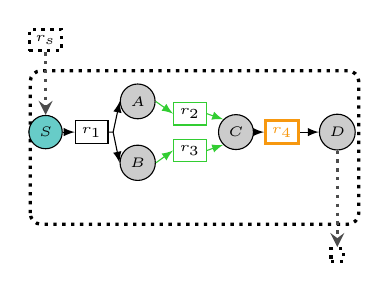
\begin{tikzpicture}[scale=0.39]\tiny
      \tikzstyle{metabolite}=[draw,circle,fill=white!80!black];
      \tikzstyle{repairmetabolite}=[draw,white!40!black, circle,fill=white!90!black,text=white!40!black,dashed];
      \tikzstyle{seed}=[draw,circle,fill=BlueGreen!70];%white!80!black
      \tikzstyle{target}=[draw,circle,fill=YellowOrange];%white!40!black
      \tikzstyle{reaction}=[draw,rectangle];
       \tikzstyle{export}=[draw,rectangle,dotted, very thick];
       \tikzstyle{exportrepair}=[draw,rectangle,dotted, very thick,white!80!black,text=white!70!black];
      \tikzstyle{repairreaction}=[draw,rectangle,white!40!black,text=white!40!black,dashed];
      \tikzstyle{solreaction}=[draw,rectangle,LimeGreen,text=black];
      \tikzstyle{initial}=[->,>=latex,thick];
      \tikzstyle{bdd}=[->,>=latex,thick];
      \tikzstyle{etiq}=[midway,fill=black!20,scale=0.5];
      \tikzstyle{stc}=[draw, rectangle, white, text=black]


      \draw [black,dotted, rounded corners, very thick] (-0.5,4) rectangle (10.2,9);
     % \node (system) [draw, rounded rectangle] at (0,0) {} (7cm,5cm);

      \node[seed] (S) at (0,7) {$S$};
      \node[metabolite] (A) at (3,8) {$A$};
      \node[metabolite] (B) at (3,6) {$B$};
      \node[metabolite] (C) at (6.2,7) {$C$};
      \node[metabolite] (D) at (9.5,7) {$D$};

      \node[reaction] (R1) at (1.5,7) {$r_{1}$};
      \node[reaction, very thick,YellowOrange] (R4) at (7.7,7) {$r_{4}$}; %LimeGreen
      \node[solreaction] (R2) at (4.7,7.6) {$r_{2}$};
      \node[solreaction] (R3) at (4.7,6.4) {$r_{3}$};

      % R1 : S => A + B
      \draw[->,>=latex] (S.east) -- (R1.west);
      \draw[->,>=latex] (R1.east) -- (2.2,7) -- (A.west);
      \draw[->,>=latex] (2.2,7)  -- (B.west);

      % R2 : A => C
      \draw[->,>=latex,LimeGreen] (A.east) -- (R2.west);
      \draw[->,>=latex,LimeGreen] (R2.east) -- (C.north west);

      % R3 : B => C
      \draw[->,>=latex,LimeGreen] (B.east) -- (R3.west);
      \draw[->,>=latex,LimeGreen] (R3.east) -- (C.south west);

      % R4 : C => D
      \draw[->,>=latex] (C.east) -- (R4.west);
      \draw[->,>=latex] (R4.east) -- (D.west);

      %export G
      \node[export] (outD) at (9.5,3) {\ExportReaction};
      \draw[->,>=stealth,white!30!black,dotted, very thick] (D.south) --  (outD.north);

      %import S2
      \node[export] (inS) at (0,10) {$r_{s}$};
      \draw[->,>=stealth,white!30!black,dotted, very thick] (inS) --  (S.north);

  \end{tikzpicture}
% \end{figure}

% \end{document}

      \caption{Completion with the union $R_1\cup R_2=\{r_2,r_3\}$. $G=G_1\cup G_2$  satisfies $r_4\in\Activity{h}{G}{\{S\}}$ and thus is flux-balanced.
      \label{gra:union_nf_f}}
    \end{minipage}
\end{figure}
% ----------------------------------------------------------------------


% ----------------------------------------------------------------------
\begin{figure}
    \captionsetup{width=0.3\textwidth}
    \centering
    \begin{minipage}[t]{.32\textwidth}
      % \documentclass{article}
% \usepackage[dvipsnames]{xcolor}
% \usepackage{tikz}
% \usepackage{xcolor,colortbl}
% 
% \begin{document}
% 
% \newcommand{\gringo}{\textit{gringo}}
\newcommand{\clasp}{\textit{clasp}}
\newcommand{\clingo}{\textit{clingo}}
\newcommand{\asprin}{\textit{asprin}}
\newcommand{\asap}{\textit{teaspoon}}
\newcommand{\piclasp}{\textit{piclasp}}

\newcommand{\code}[1]{\lstinline[basicstyle=\ttfamily]{#1}}

\newcommand{\lw}[1]{\smash{\lower1.ex\hbox{#1}}}
\newcommand{\llw}[1]{\smash{\lower3.ex\hbox{#1}}}

%\newcommand{\dataCL}[5]{%
%  \code{#1} & #3 & #5 & #4
%}
%\newcommand{\dataCS}[5]{%
%  #3 & #5 & #4
%}

\newenvironment{tableC}{%
  \scriptsize
  \tabcolsep = 0.6mm
  \begin{tabular}[t]{l|rlr|rlr|rlr|rlr|rlr}\hline
    \multicolumn{1}{l|}{\llw{Instance}} &
    \multicolumn{3}{c|}{UD1} &
    \multicolumn{3}{c|}{UD2} &
    \multicolumn{3}{c|}{UD3} &
    \multicolumn{3}{c|}{UD4} &
    \multicolumn{3}{c}{UD5} \\
    & 
    \multicolumn{1}{c}{Best} & & \multicolumn{1}{c|}{\emph{tea-}} & 
    \multicolumn{1}{c}{Best} & & \multicolumn{1}{c|}{\emph{tea-}} & 
    \multicolumn{1}{c}{Best} & & \multicolumn{1}{c|}{\emph{tea-}} & 
    \multicolumn{1}{c}{Best} & & \multicolumn{1}{c|}{\emph{tea-}} & 
    \multicolumn{1}{c}{Best} & & \multicolumn{1}{c}{\emph{tea-}} \\
    & 
    known & & \emph{spoon} & 
    known & & \emph{spoon} & 
    known & & \emph{spoon} & 
    known & & \emph{spoon} & 
    known & & \emph{spoon} \\
    \hline
  }{%
    \hline
  \end{tabular}
}

\newenvironment{tableB}{%
  \scriptsize
  \tabcolsep = 0.7mm
%  \begin{tabular}[t]{|l|c|r|l|l|l|}\hline
  \begin{tabular}[t]{lcrlll}\hline
    Instance &
    Formulation &
    Time (sec.)\\
    \hline
  }{%
    \hline
  \end{tabular}
}
\newenvironment{tableL}{%
  \scriptsize
  \tabcolsep = 0.7mm
  \begin{tabular}[t]{l|rrrrrrrr|r}\hline
    \lw{Instance} &
    \lw{Time (sec.)} &
    \multicolumn{6}{c}{The best utility vector} &
    The sum of  &
    The best of basic\\
    &
    &
    $(S_1,$ & $S_4,$ & $S_2,$ & $S_7,$ & $S_6,$ & $S_3)$ &
    utility vector &
    and optimized \\
    \hline
  }{%
    \hline
  \end{tabular}
}

%%% Local Variables:
%%% mode: latex
%%% TeX-master: "paper"
%%% End:


% \begin{figure}[t]
%   \centering

    \usetikzlibrary{shapes.misc, positioning}
    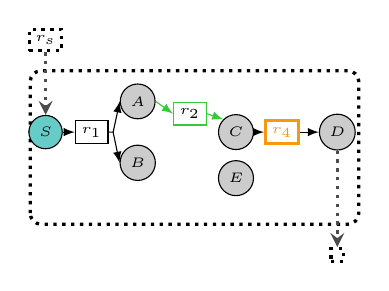
\begin{tikzpicture}[scale=0.39]\tiny
      \tikzstyle{metabolite}=[draw,circle,fill=white!80!black];
      \tikzstyle{repairmetabolite}=[draw,white!40!black, circle,fill=white!90!black,text=white!40!black,dashed];
      \tikzstyle{seed}=[draw,circle,fill=BlueGreen!70];%white!80!black
      \tikzstyle{target}=[draw,circle,fill=YellowOrange];%white!40!black
      \tikzstyle{reaction}=[draw,rectangle];
       \tikzstyle{export}=[draw,rectangle,dotted, very thick];
       \tikzstyle{exportrepair}=[draw,rectangle,dotted, very thick,white!80!black,text=white!70!black];
      \tikzstyle{repairreaction}=[draw,rectangle,white!40!black,text=white!40!black,dashed];
      \tikzstyle{solreaction}=[draw,rectangle,LimeGreen,text=black];
      \tikzstyle{initial}=[->,>=latex,thick];
      \tikzstyle{bdd}=[->,>=latex,thick];
      \tikzstyle{etiq}=[midway,fill=black!20,scale=0.5];
      \tikzstyle{stc}=[draw, rectangle, white, text=black]


      \draw [black,dotted, rounded corners, very thick] (-0.5,4) rectangle (10.2,9);
     % \node (system) [draw, rounded rectangle] at (0,0) {} (7cm,5cm);

      \node[seed] (S) at (0,7) {$S$};
      \node[metabolite] (A) at (3,8) {$A$};
      \node[metabolite] (B) at (3,6) {$B$};
      \node[metabolite] (C) at (6.2,7) {$C$};
      \node[metabolite] (D) at (9.5,7) {$D$};
      \node[metabolite] (E) at (6.2,5.5) {$E$};

      \node[reaction] (R1) at (1.5,7) {$r_{1}$};
      \node[reaction, very thick,YellowOrange] (R4) at (7.7,7) {$r_{4}$}; %LimeGreen
      \node[solreaction] (R2) at (4.7,7.6) {$r_{2}$};
      %\node[solreaction] (R3) at (4.7,6.4) {$r_{3}$};

      % R1 : S => A + B
      \draw[->,>=latex] (S.east) -- (R1.west);
      \draw[->,>=latex] (R1.east) -- (2.2,7) -- (A.west);
      \draw[->,>=latex] (2.2,7)  -- (B.west);

      % R2 : A => C
      \draw[->,>=latex,LimeGreen] (A.east) -- (R2.west);
      \draw[->,>=latex,LimeGreen] (R2.east) -- (C.north west);

      % R3 : B => C + E
      %\draw[->,>=latex,LimeGreen] (B.east) -- (R3.west);
      %\draw[->,>=latex,LimeGreen] (R3.east) -- (C.south west);
      %\draw[->,>=latex,LimeGreen] (R3.east) -- (E.west);

      % R4 : C => D
      \draw[->,>=latex] (C.east) -- (R4.west);
      \draw[->,>=latex] (R4.east) -- (D.west);

      %export G
      \node[export] (outD) at (9.5,3) {\ExportReaction};
      \draw[->,>=stealth,white!30!black,dotted, very thick] (D.south) --  (outD.north);

      %import S2
      \node[export] (inS) at (0,10) {$r_{s}$};
      \draw[->,>=stealth,white!30!black,dotted, very thick] (inS) --  (S.north);

  \end{tikzpicture}
% \end{figure}

% \end{document}

      \caption{Topological completion $R_1=\{r_2\}$ satisfies $r_4\in\Activity{t}{G_1}{\{S\}}$, but carries no flux, due to accumulation of compound $B$ that contradicts Eq.~\ref{eq:stoichiometric:equation}.\label{gra:union_nf_nf1}}
    \end{minipage}
    \begin{minipage}[t]{.32\textwidth}
      % \documentclass{article}
% \usepackage[dvipsnames]{xcolor}
% \usepackage{tikz}
% \usepackage{xcolor,colortbl}
% 
% \begin{document}
% 
% \newcommand{\gringo}{\textit{gringo}}
\newcommand{\clasp}{\textit{clasp}}
\newcommand{\clingo}{\textit{clingo}}
\newcommand{\asprin}{\textit{asprin}}
\newcommand{\asap}{\textit{teaspoon}}
\newcommand{\piclasp}{\textit{piclasp}}

\newcommand{\code}[1]{\lstinline[basicstyle=\ttfamily]{#1}}

\newcommand{\lw}[1]{\smash{\lower1.ex\hbox{#1}}}
\newcommand{\llw}[1]{\smash{\lower3.ex\hbox{#1}}}

%\newcommand{\dataCL}[5]{%
%  \code{#1} & #3 & #5 & #4
%}
%\newcommand{\dataCS}[5]{%
%  #3 & #5 & #4
%}

\newenvironment{tableC}{%
  \scriptsize
  \tabcolsep = 0.6mm
  \begin{tabular}[t]{l|rlr|rlr|rlr|rlr|rlr}\hline
    \multicolumn{1}{l|}{\llw{Instance}} &
    \multicolumn{3}{c|}{UD1} &
    \multicolumn{3}{c|}{UD2} &
    \multicolumn{3}{c|}{UD3} &
    \multicolumn{3}{c|}{UD4} &
    \multicolumn{3}{c}{UD5} \\
    & 
    \multicolumn{1}{c}{Best} & & \multicolumn{1}{c|}{\emph{tea-}} & 
    \multicolumn{1}{c}{Best} & & \multicolumn{1}{c|}{\emph{tea-}} & 
    \multicolumn{1}{c}{Best} & & \multicolumn{1}{c|}{\emph{tea-}} & 
    \multicolumn{1}{c}{Best} & & \multicolumn{1}{c|}{\emph{tea-}} & 
    \multicolumn{1}{c}{Best} & & \multicolumn{1}{c}{\emph{tea-}} \\
    & 
    known & & \emph{spoon} & 
    known & & \emph{spoon} & 
    known & & \emph{spoon} & 
    known & & \emph{spoon} & 
    known & & \emph{spoon} \\
    \hline
  }{%
    \hline
  \end{tabular}
}

\newenvironment{tableB}{%
  \scriptsize
  \tabcolsep = 0.7mm
%  \begin{tabular}[t]{|l|c|r|l|l|l|}\hline
  \begin{tabular}[t]{lcrlll}\hline
    Instance &
    Formulation &
    Time (sec.)\\
    \hline
  }{%
    \hline
  \end{tabular}
}
\newenvironment{tableL}{%
  \scriptsize
  \tabcolsep = 0.7mm
  \begin{tabular}[t]{l|rrrrrrrr|r}\hline
    \lw{Instance} &
    \lw{Time (sec.)} &
    \multicolumn{6}{c}{The best utility vector} &
    The sum of  &
    The best of basic\\
    &
    &
    $(S_1,$ & $S_4,$ & $S_2,$ & $S_7,$ & $S_6,$ & $S_3)$ &
    utility vector &
    and optimized \\
    \hline
  }{%
    \hline
  \end{tabular}
}

%%% Local Variables:
%%% mode: latex
%%% TeX-master: "paper"
%%% End:


% \begin{figure}[t]
%   \centering

    \usetikzlibrary{shapes.misc, positioning}
    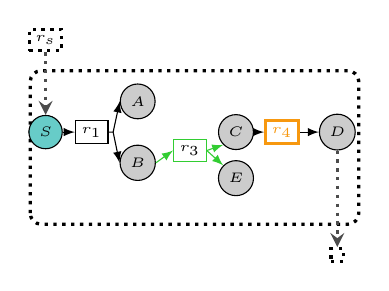
\begin{tikzpicture}[scale=0.39]\tiny
      \tikzstyle{metabolite}=[draw,circle,fill=white!80!black];
      \tikzstyle{repairmetabolite}=[draw,white!40!black, circle,fill=white!90!black,text=white!40!black,dashed];
      \tikzstyle{seed}=[draw,circle,fill=BlueGreen!70];%white!80!black
      \tikzstyle{target}=[draw,circle,fill=YellowOrange];%white!40!black
      \tikzstyle{reaction}=[draw,rectangle];
       \tikzstyle{export}=[draw,rectangle,dotted, very thick];
       \tikzstyle{exportrepair}=[draw,rectangle,dotted, very thick,white!80!black,text=white!70!black];
      \tikzstyle{repairreaction}=[draw,rectangle,white!40!black,text=white!40!black,dashed];
      \tikzstyle{solreaction}=[draw,rectangle,LimeGreen,text=black];
      \tikzstyle{initial}=[->,>=latex,thick];
      \tikzstyle{bdd}=[->,>=latex,thick];
      \tikzstyle{etiq}=[midway,fill=black!20,scale=0.5];
      \tikzstyle{stc}=[draw, rectangle, white, text=black]


      \draw [black,dotted, rounded corners, very thick] (-0.5,4) rectangle (10.2,9);
     % \node (system) [draw, rounded rectangle] at (0,0) {} (7cm,5cm);

      \node[seed] (S) at (0,7) {$S$};
      \node[metabolite] (A) at (3,8) {$A$};
      \node[metabolite] (B) at (3,6) {$B$};
      \node[metabolite] (C) at (6.2,7) {$C$};
      \node[metabolite] (D) at (9.5,7) {$D$};
      \node[metabolite] (E) at (6.2,5.5) {$E$};

      \node[reaction] (R1) at (1.5,7) {$r_{1}$};
      \node[reaction, very thick,YellowOrange] (R4) at (7.7,7) {$r_{4}$}; %LimeGreen
      %\node[solreaction] (R2) at (4.7,7.6) {$r_{2}$};
      \node[solreaction] (R3) at (4.7,6.4) {$r_{3}$};

      % R1 : S => A + B
      \draw[->,>=latex] (S.east) -- (R1.west);
      \draw[->,>=latex] (R1.east) -- (2.2,7) -- (A.west);
      \draw[->,>=latex] (2.2,7)  -- (B.west);

      % R2 : A => C
      %\draw[->,>=latex,LimeGreen] (A.east) -- (R2.west);
      %\draw[->,>=latex,LimeGreen] (R2.east) -- (C.north west);

      % R3 : B => C + E
      \draw[->,>=latex,LimeGreen] (B.east) -- (R3.west);
      \draw[->,>=latex,LimeGreen] (R3.east) -- (C.south west);
      \draw[->,>=latex,LimeGreen] (R3.east) -- (E.north west);

      % R4 : C => D
      \draw[->,>=latex] (C.east) -- (R4.west);
      \draw[->,>=latex] (R4.east) -- (D.west);

      %export G
      \node[export] (outD) at (9.5,3) {\ExportReaction};
      \draw[->,>=stealth,white!30!black,dotted, very thick] (D.south) --  (outD.north);

      %import S2
      \node[export] (inS) at (0,10) {$r_{s}$};
      \draw[->,>=stealth,white!30!black,dotted, very thick] (inS) --  (S.north);

  \end{tikzpicture}
% \end{figure}

% \end{document}

      \caption{Topological completion $R_1=\{r_3\}$ satisfies $r_4\in\Activity{t}{G_2}{\{S\}}$, but carries no flux, due to accumulation of compounds $A$ and $E$ that contradicts Eq.~\ref{eq:stoichiometric:equation}.\label{gra:union_nf_nf2}}
    \end{minipage}
    \begin{minipage}[t]{.32\textwidth}
      % \documentclass{article}
% \usepackage[dvipsnames]{xcolor}
% \usepackage{tikz}
% \usepackage{xcolor,colortbl}
% 
% \begin{document}
% 
% \newcommand{\gringo}{\textit{gringo}}
\newcommand{\clasp}{\textit{clasp}}
\newcommand{\clingo}{\textit{clingo}}
\newcommand{\asprin}{\textit{asprin}}
\newcommand{\asap}{\textit{teaspoon}}
\newcommand{\piclasp}{\textit{piclasp}}

\newcommand{\code}[1]{\lstinline[basicstyle=\ttfamily]{#1}}

\newcommand{\lw}[1]{\smash{\lower1.ex\hbox{#1}}}
\newcommand{\llw}[1]{\smash{\lower3.ex\hbox{#1}}}

%\newcommand{\dataCL}[5]{%
%  \code{#1} & #3 & #5 & #4
%}
%\newcommand{\dataCS}[5]{%
%  #3 & #5 & #4
%}

\newenvironment{tableC}{%
  \scriptsize
  \tabcolsep = 0.6mm
  \begin{tabular}[t]{l|rlr|rlr|rlr|rlr|rlr}\hline
    \multicolumn{1}{l|}{\llw{Instance}} &
    \multicolumn{3}{c|}{UD1} &
    \multicolumn{3}{c|}{UD2} &
    \multicolumn{3}{c|}{UD3} &
    \multicolumn{3}{c|}{UD4} &
    \multicolumn{3}{c}{UD5} \\
    & 
    \multicolumn{1}{c}{Best} & & \multicolumn{1}{c|}{\emph{tea-}} & 
    \multicolumn{1}{c}{Best} & & \multicolumn{1}{c|}{\emph{tea-}} & 
    \multicolumn{1}{c}{Best} & & \multicolumn{1}{c|}{\emph{tea-}} & 
    \multicolumn{1}{c}{Best} & & \multicolumn{1}{c|}{\emph{tea-}} & 
    \multicolumn{1}{c}{Best} & & \multicolumn{1}{c}{\emph{tea-}} \\
    & 
    known & & \emph{spoon} & 
    known & & \emph{spoon} & 
    known & & \emph{spoon} & 
    known & & \emph{spoon} & 
    known & & \emph{spoon} \\
    \hline
  }{%
    \hline
  \end{tabular}
}

\newenvironment{tableB}{%
  \scriptsize
  \tabcolsep = 0.7mm
%  \begin{tabular}[t]{|l|c|r|l|l|l|}\hline
  \begin{tabular}[t]{lcrlll}\hline
    Instance &
    Formulation &
    Time (sec.)\\
    \hline
  }{%
    \hline
  \end{tabular}
}
\newenvironment{tableL}{%
  \scriptsize
  \tabcolsep = 0.7mm
  \begin{tabular}[t]{l|rrrrrrrr|r}\hline
    \lw{Instance} &
    \lw{Time (sec.)} &
    \multicolumn{6}{c}{The best utility vector} &
    The sum of  &
    The best of basic\\
    &
    &
    $(S_1,$ & $S_4,$ & $S_2,$ & $S_7,$ & $S_6,$ & $S_3)$ &
    utility vector &
    and optimized \\
    \hline
  }{%
    \hline
  \end{tabular}
}

%%% Local Variables:
%%% mode: latex
%%% TeX-master: "paper"
%%% End:


% \begin{figure}[t]
%   \centering

    \usetikzlibrary{shapes.misc, positioning}
    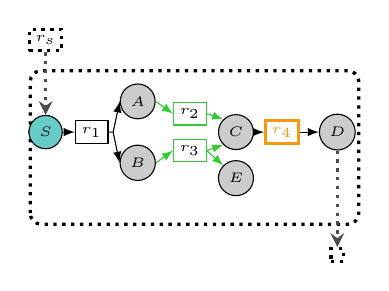
\begin{tikzpicture}[scale=0.39]\tiny
      \tikzstyle{metabolite}=[draw,circle,fill=white!80!black];
      \tikzstyle{repairmetabolite}=[draw,white!40!black, circle,fill=white!90!black,text=white!40!black,dashed];
      \tikzstyle{seed}=[draw,circle,fill=BlueGreen!70];%white!80!black
      \tikzstyle{target}=[draw,circle,fill=YellowOrange];%white!40!black
      \tikzstyle{reaction}=[draw,rectangle];
       \tikzstyle{export}=[draw,rectangle,dotted, very thick];
       \tikzstyle{exportrepair}=[draw,rectangle,dotted, very thick,white!80!black,text=white!70!black];
      \tikzstyle{repairreaction}=[draw,rectangle,white!40!black,text=white!40!black,dashed];
      \tikzstyle{solreaction}=[draw,rectangle,LimeGreen,text=black];
      \tikzstyle{initial}=[->,>=latex,thick];
      \tikzstyle{bdd}=[->,>=latex,thick];
      \tikzstyle{etiq}=[midway,fill=black!20,scale=0.5];
      \tikzstyle{stc}=[draw, rectangle, white, text=black]


      \draw [black,dotted, rounded corners, very thick] (-0.5,4) rectangle (10.2,9);
     % \node (system) [draw, rounded rectangle] at (0,0) {} (7cm,5cm);

      \node[seed] (S) at (0,7) {$S$};
      \node[metabolite] (A) at (3,8) {$A$};
      \node[metabolite] (B) at (3,6) {$B$};
      \node[metabolite] (C) at (6.2,7) {$C$};
      \node[metabolite] (D) at (9.5,7) {$D$};
      \node[metabolite] (E) at (6.2,5.5) {$E$};

      \node[reaction] (R1) at (1.5,7) {$r_{1}$};
      \node[reaction, very thick,YellowOrange] (R4) at (7.7,7) {$r_{4}$}; %LimeGreen
      \node[solreaction] (R2) at (4.7,7.6) {$r_{2}$};
      \node[solreaction] (R3) at (4.7,6.4) {$r_{3}$};

      % R1 : S => A + B
      \draw[->,>=latex] (S.east) -- (R1.west);
      \draw[->,>=latex] (R1.east) -- (2.2,7) -- (A.west);
      \draw[->,>=latex] (2.2,7)  -- (B.west);

      % R2 : A => C
      \draw[->,>=latex,LimeGreen] (A.east) -- (R2.west);
      \draw[->,>=latex,LimeGreen] (R2.east) -- (C.north west);

      % R3 : B => C + E
      \draw[->,>=latex,LimeGreen] (B.east) -- (R3.west);
      \draw[->,>=latex,LimeGreen] (R3.east) -- (C.south west);
      \draw[->,>=latex,LimeGreen] (R3.east) -- (E.north west);

      % R4 : C => D
      \draw[->,>=latex] (C.east) -- (R4.west);
      \draw[->,>=latex] (R4.east) -- (D.west);

      %export G
      \node[export] (outD) at (9.5,3) {\ExportReaction};
      \draw[->,>=stealth,white!30!black,dotted, very thick] (D.south) --  (outD.north);

      %import S2
      \node[export] (inS) at (0,10) {$r_{s}$};
      \draw[->,>=stealth,white!30!black,dotted, very thick] (inS) --  (S.north);

  \end{tikzpicture}
% \end{figure}

% \end{document}

      \caption{Completion with the union $R_1\cup R_2=\{r_2,r_3\}$. $G=G_1\cup G_2$ satisfies $r_4\in\Activity{t}{G}{\{S\}}$, but contradicts minimality and carries no flux $r_4\not \in\Activity{s}{G}{\{S\}}$, due to accumulation of compound $E$ that contradicts Eq.~\ref{eq:stoichiometric:equation}.\label{gra:union_nf_nf}}
    \end{minipage}
\end{figure}
% ----------------------------------------------------------------------



%%% Local Variables:
%%% mode: latex
%%% TeX-master: "paper"
%%% End:

\section{Curriculum-based Course Timetabling}\label{sec:cb-ctt}

As mentioned, we focus on the curriculum-based course timetabling
(CB-CTT) problems used in the ITC-2007 competition.
The problem description of CB-CTT presented here is based on 
\citep{DBLP:journals/anor/BonuttiCGS12}.

The CB-CTT instance consists mainly of
\textit{curricula},
\textit{courses},
\textit{rooms},
\textit{days}, and
\textit{periods} per day.
A curriculum is a set of courses that shares common students.
We refer to a pair of day and period as \textit{timeslot}.
%
The CB-CTT problem is defined as the task of assigning all lectures
of each course into a weekly timetable, 
subject to a given set of hard and soft constraints.
%
Hard constraints must be strictly satisfied.
Soft constraints are not necessarily satisfied,
but the sum of their violations should be minimal.
%
A \textit{feasible solution} of the problem is an assignment
so that the hard constraints are satisfied.
The objective of the problem is to find a feasible solution with minimal penalty.
%
The CB-CTT problem has the following hard constraints.
\begin{list}{}{}
\item \bm{$H_1$}. \textbf{Lectures}: 
  All lectures of each course must be scheduled, 
  and they must be assigned to distinct timeslots.
\item \bm{$H_2$}. \textbf{Conflicts}: 
  Lectures of courses in the same curriculum or taught by the same
  teacher must be all scheduled in different timeslots.
\item \bm{$H_3$}. \textbf{RoomOccupancy}: 
  Two lectures cannot take place in the same room in the same timeslot.
\item \bm{$H_4$}. \textbf{Availability}: 
  If the teacher of the course is unavailable to teach that course
  at a given timeslot, then no lecture of the course can be scheduled at
  that timeslot.
\end{list}
The CB-CTT problem has the following soft constraints.
\begin{list}{}{}
\item\bm{$S_1$}. \textbf{RoomCapacity}: 
  For each lecture, the number of students that attend the course must
  be less than or equal the number of seats of all the rooms that host
  its lectures. 
  The penalty points, reflecting the number of students above the
  capacity, are imposed on each violation.
\item\bm{$S_2$}. \textbf{MinWorkingDays}: 
  The lectures of each course must be spread into a given minimum
  number of days. 
  The penalty points, reflecting the number of days below the minimum,
  are imposed on each violation.
\item\bm{$S_3$}. \textbf{IsolatedLectures}: 
  Lectures belonging to a curriculum should be adjacent to each other
  in consecutive timeslots. For a given curriculum we account
  for a violation every time there is one lecture not adjacent to any
  other lecture within the same day. 
  Each isolated lecture in a curriculum counts as 1 violation.
\item\bm{$S_4$}. \textbf{Windows}: 
  Lectures belonging to a curriculum should not have time windows
  (periods without teaching) between them. 
  For a given
  curriculum we account for a violation every time there is one
  window between two lectures within the same day. 
  The penalty points, reflecting the length in periods of time window,
  are imposed on each violation.
\item\bm{$S_5$}. \textbf{RoomStability}: 
  All lectures of a course should be given in the same room. 
  The penalty points, reflecting the number of distinct rooms but the first, 
  are imposed on each violation.
\item\bm{$S_6$}. \textbf{StudentMinMaxLoad}: 
  For each curriculum the number of daily lectures should be within a
  given range. 
  The penalty points, reflecting the number of lectures below the minimum or above the
  maximum, are imposed on each violation.
\item\bm{$S_7$}. \textbf{TravelDistance}: 
  Students should have the time to move from one building to another
  one between two lectures. For a given curriculum we account for a
  violation every time there is an \textit{instantaneous move}: 
  two lectures in rooms located in different building in two adjacent
  periods within the same day. 
  Each instantaneous move in a curriculum counts as 1 violation.
\item\bm{$S_8$}. \textbf{RoomSuitability}:
  Some rooms may be not suitable for a given course because of the
  absence of necessary equipment.
  Each lecture of a course in an unsuitable room counts as 1
  violation.
\item\bm{$S_9$}. \textbf{DoubleLectures}:
  Some courses require that lectures in the same day are grouped
  together (\textit{double lectures}). For a course that requires grouped
  lectures, every time there is more than one lecture in one day, 
  a lecture non-grouped to another is not allowed. 
  Two lectures are grouped if they are adjacent and in the same room. 
  Each non-grouped lecture counts as 1 violation.
\end{list}

%%%%%%%%%%%%%%%%%%%%%%%%%%%%%%%%%%%%%%%%%%%%
\begin{table}
\centering
\caption{Problem Formulations}
\label{table:problem_formulations}
%\renewcommand{\arraystretch}{0.9}
%\tabcolsep = 3mm
\begin{tabular}[t]{l|ccccc}\hline
Constraint & UD1 & UD2 & UD3 & UD4 & UD5\\\hline
$H_1$. Lectures &  
H &  H &  H &  H & H\\
$H_2$. Conflicts &  
H &  H &  H &  H & H\\
$H_3$. RoomOccupancy &  
H &  H &  H &  H & H\\
$H_4$. Availability &  
H &  H &  H &  H & H\\
$S_1$. RoomCapacity &  
1 & 1 & 1 & 1  & 1 \\
$S_2$. MinWorkingDays &  
5 &  5 & - & 1 & 5 \\
$S_3$. IsolatedLectures &  
1 & 2 & - & - & 1 \\
$S_4$. Windows &  
- & - & 4 & 1 & 2\\
$S_5$. RoomStability &  
- & 1 & - & - & -\\
$S_6$. StudentMinMaxLoad &  
- & - & 2 & 1 & 2\\
$S_7$. TravelDistance &  
- & - & - & - & 2\\
$S_8$. RoomSuitability &  
- & - & 3 & H & -\\
$S_9$. DoubleLectures &  
- & - & - & 1 & -\\\hline
\end{tabular}
\end{table}
%%%%%%%%%%%%%%%%%%%%%%%%%%%%%%%%%%%%%%%%%%%%

A \textit{formulation} is defined as a specific set of soft constraints
together with the weights associated with each of them.
%
The five formulations UD1--UD5 have been proposed so far.
UD1 is the most basic formulation among them~\citep{DBLP:conf/patat/GasperoS02}.
UD2 is a well known formulation used in the ITC-2007 competition~\citep{GasperoMS/ITC2007}.
UD3, UD4, and UD5 have been recently proposed
to capture more different scenarios~\citep{DBLP:journals/anor/BonuttiCGS12}.
These formulations focus on 
student load (UD3), 
double lectures (UD4), and
travel cost (UD5), respectively.
%
The weights of soft constraints in each formulation is shown in 
Table~\ref{table:problem_formulations}.
The symbol `H' stands for inclusion in a formulation as hard constraint.
The symbol `-' stands for exclusion from a formulation.

In this paper, we formulate the CB-CTT problem as a single-objective
combinatorial optimization problem whose objective function is to
minimize the weighted sum of penalty points in the same manner as
ITC-2007, 
as well as a multi-criteria optimization problem based on lexicographic ordering.
Furthermore, we consider a multi-objective course timetabling problem
combining CB-CTT and Minimal Perturbation Problem.

%%% Local Variables:
%%% mode: latex
%%% TeX-master: "paper"
%%% End:


\section{The {\asap} Approach}\label{sec:approach}

We begin with describing {\asap}'s fact format of CB-CTT instances and
then present a basic {\asap} encoding for solving the CB-CTT problems
\footnote{{\asap}: \textbf{T}im\textbf{E}tabling with \textbf{A}nswer \textbf{S}et \textbf{P}r\textbf{O}grammi\textbf{N}g}.
%%%%%%%%%%%%%%%%%%%%%%%%%
\subsection{Fact Format}
%\textbf{Fact Format.}
%%%%%%%%%%%%%%%%%%%%%%%%%
\begin{figure}[t]
\centering
\begin{minipage}[t]{.45\textwidth}
\lstinputlisting[caption={A toy instance of the \code{ectt} format},%
captionpos=b,frame=single,label=ex:toy.ectt,%
numbers=none,%
basicstyle=\ttfamily\scriptsize]{code_toy1_ectt.tex}
\end{minipage}\hfill
\begin{minipage}[t]{.45\textwidth}
\lstinputlisting[frame=single,numbers=none,%
basicstyle=\ttfamily\scriptsize]{code_toy2_ectt.tex}
\end{minipage}
\end{figure}
%
\lstinputlisting[float=t,caption={ASP facts representing the toy instance of Listing~\ref{ex:toy.ectt}},%
captionpos=b,frame=single,label=ex:toy.lp,%
%numbers=none,%
breaklines=true,%
columns=fullflexible,keepspaces=true,%
basicstyle=\ttfamily\scriptsize]{code_toy_lp.tex}
%
\lstinputlisting[float=t,caption={Solution (partial answer set) of the toy instance in UD2},%
captionpos=b,frame=single,label=ex:toy_out.lp,%
%numbers=none,%
breaklines=true,%
columns=fullflexible,keepspaces=true,%
basicstyle=\ttfamily\scriptsize]{code_toy_sol_lp.tex}
%%%%%%%%%%%%%%%%%%%%%%%%%
Listing~\ref{ex:toy.ectt} shows a toy instance of the \code{ectt}
format, which is a standard input format of CB-CTT 
instances~\citep{DBLP:journals/anor/BonuttiCGS12}.
The format has headers that represent basic entities, followed
by five blocks, 
\code{COURSES}, 
\code{ROOMS}, 
\code{CURRICULA}, 
\code{UNAVAILABILITY_CONSTRAINTS}, and 
\code{ROOM_CONSTRAINTS}.

ASP facts representing the toy instance are shown in
Listing~\ref{ex:toy.lp}.
There exists a one-to-one correspondence between ASP fact format and
the \code{ectt} format except for the \code{CURRICULA} block.
%
The facts in Line 1--2 correspond to the \code{ectt} headers and
express that
the instance named \texttt{Toy} consists of 
4 courses, 
3 rooms,
2 curricula,
8 unavailability constraints, and 
3 room constraints.
The weekly timetable consists of 
5 days and 4 periods per day, which start from 0.
The fact \code{min_max_daily_lectures(2,3)} expresses 
the minimum and maximum numbers of daily lectures 
for each curriculum, and is used to specify $S_6$.

Each fact of predicate \code{course/6} in Line 4--5
corresponds to a line of the \code{COURSES} block.
A fact \texttt{course($C$,$T$,$N$,$MWD$,$M$,$DL$)}
expresses that a course $C$ taught by a teacher $T$ 
consists of $N$ lectures, which must be spread into $MWD$ days.  
The number of students attending the course $C$ is $M$.  
The course $C$ requires double lectures if $DL=1$.  
%
Each fact of predicate \code{room/3} in Line 7 
corresponds to a line of the \code{ROOMS} block.
A fact \texttt{room($R$,$CAP$,$BLD$)} expresses that a
room $R$ in a building $BLD$ has a seating capacity of $CAP$.

A fact \texttt{curricula($CUR$, $C$)} in Line 9--10 expresses that
a course $C$ belongs to a curriculum $CUR$.
%
Each fact of predicate \code{unavailability_constraint/3} in Line
12--15 corresponds to a line of the 
\code{UNAVAILABILITY_CONSTRAINTS} block, and is used to specify $H_4$.
A fact \texttt{unavailability\_constraint($C$,$D$,$P$)}
expresses that a course $C$ is not available at a period $P$ on a day
$D$.
%
Each fact of predicate \code{room_constraint/2} in Line 17
corresponds to a line of the \code{ROOM_CONSTRAINTS} block, and
is used to specify $S_8$.
A fact \texttt{room\_constraint($C$,$R$)} expresses that a room $R$ is
not suitable for a course $C$.

Listing~\ref{ex:toy_out.lp} shows an optimal solution with zero penalty
of the toy instance in the UD2 formulation.
Each atom \texttt{assigned($C$,$R$,$D$,$P$)} is intended to
express that a lecture of a course $C$ is assigned to 
a room $R$ at a period $P$ on a day $D$.
We can observe from Line 1 that
the lectures of the course \texttt{SceCosC} are
assigned to the room \texttt{rB} at
the first period (\texttt{0}) on Thursday (\texttt{3}),
the third period (\texttt{2}) on Wednesday (\texttt{2}), and
the third period (\texttt{2}) on Friday (\texttt{4})


\subsection{First-Order Encoding}
%\textbf{First-Order Encoding.}
%%%%%%%%%%%%%%%%%%%%%%%%%
\lstinputlisting[float=t,caption={Encoding of hard constraints},%
captionpos=b,frame=single,label=en:ctt_hard2.lp4,%
%numbers=none,%
breaklines=true,%
columns=fullflexible,keepspaces=true,%
basicstyle=\ttfamily\scriptsize]{code_hard_lp.tex}
%%%%%%%%%%%%%%%%%%%%%%%%%
\lstinputlisting[float=t,caption={Encoding of soft constraints and objective function},%
captionpos=b,frame=single,label=en:ctt_soft.lp4,%
%numbers=none,%
breaklines=true,%
columns=fullflexible,keepspaces=true,%
basicstyle=\ttfamily\scriptsize]{code_soft_lp.tex}
%%%%%%%%%%%%%%%%%%%%%%%%%
The {\asap} encoding of hard constraints ($H_1$--$H_4$) is shown in 
Listing~\ref{en:ctt_hard2.lp4}.
The expressive power of ASP's modelling language enables us to express
each hard constraint individually by just one or two ASP rules.
%
As mentioned, the atom \texttt{assigned($C$,$R$,$D$,$P$)}
expresses that a lecture of a course $C$ is assigned to a room $R$ at
a period $P$ on a day $D$, and a solution is composed of 
a set of these assignments.
The atom \texttt{assigned($C$,$D$,$P$)} dropping $R$
from \texttt{assigned($C$,$R$,$D$,$P$)} is also introduced,
since we do not always have to take the room information into account 
to specify the hard constraints except $H_3$.

Given an instance expressed in our fact format,
the first four rules in Line 1--2 generate 
\code{c(C)}, 
\code{t(T)}, 
\code{r(R)}, and
\code{cu(Cu)} 
for each course \code{C}, teacher \code{T}, room \code{R}, and 
curriculum \code{Cu}.
%
The next two rules in Line 3 generate 
\code{d(0)} $\ldots$ \code{d(D-1)} and
\code{ppd(0)} $\ldots$ \code{ppd(P-1)} 
expressing that the days range from \code{0} to \code{D-1}, 
and the periods per day range from \code{0} to \code{P-1}.

For $H_1$,
the rule in Line 6,
for every course \code{C} having \code{N} lectures,
generates a set of candidate assignments
subject to the condition that 
there are exactly \code{N} lectures such that \code{assigned(C,D,P)} holds.

For $H_2$,
the rule in Line 9 enforces that,
for every teacher \code{T}, day \code{D}, and period \code{P},
there is at most one course \code{C} taught by \code{T}
such that \code{assigned(C,D,P)} holds.
In detail, 
if \code{t(T)}, \code{d(D)}, and \code{ppd(P)} hold,
this integrity constraint tells us that
the at-most-one constraint represented by 
`\verb+{ assigned(C,D,P) : course(C,T,_,_,_,_) } 1+'
must be true as well in order to prevent its body from being satisfied. 
In the similar way,
the rule in Line 10 enforces that,
for every curriculum \code{Cu}, day \code{D}, and period \code{P},
there is at most one course \code{C} that belongs to \code{Cu}
such that \code{assigned(C,D,P)} holds.

For $H_3$, 
if \code{assigned(C,D,P)} holds, 
the rule in Line 13 generates a solution candidate 
subject to the condition that there is exactly one room \code{R} such
that \code{assigned(C,R,D,P)} holds. 
The rule in Line 14 enforces that,
for every room \code{R}, day \code{D}, and period \code{P},
there is at most one course \code{C} such that 
\code{assigned(C,R,D,P)} holds.

For $H_4$,
the rule in Line 17 enforces that
a course \code{C} is not assigned at a period \code{P} on a day \code{D}
if \code{unavailability_constraint(C,D,P)} holds, since
the conjunction of literals in its body must not hold. 

The rule in Line 20 expresses that 
for each timeslot (\code{D} and \code{P})
the number of lectures assigned must be less than or equal to 
the number of rooms (\code{N}).
This rule is an implied constraint and can be omitted, but we keep it
as an additional rule for performance improvement of some problem
instances.

The {\asap} encoding of soft constraints ($S_1$--$S_9$) and an
objective function is shown in Listing~\ref{en:ctt_soft.lp4}.
We introduce a \textit{penalty atom}
\texttt{penalty($S_i$,$V$,$C$)}, which is intended to express
that a constraint $S_i$ is violated by $V$ and its penalty cost is $C$.
The constants denoted by \code{weight_of_*} indicate
the weights associated with each soft constraint defined in
Table~\ref{table:problem_formulations}.
%
Once again, each soft constraint $S_i$ is compactly expressed by
just one or two ASP rules in which the head is of the form
\texttt{penalty($S_i$,$V$,$C$)}, and a violation $V$ and its penalty
cost $C$ are detected and calculated respectively in the body.
That is, for each violation $V$ of $S_i$, 
an atom \texttt{penalty($S_i$,$V$,$C$)} is generated.
Optimal solutions can be obtained by
minimizing the number of penalty atoms in Line 49.

We explain $S_{1}$--$S_{3}$ that compose the basic UD1 formulation.
%
For $S_1$, 
the rule in Line 2--3,
for every course \code{C} that \code{N} students attend and
room \code{R} that has a seating capacity of \code{Cap},
generates a penalty atom with the cost of 
\code{(N-Cap)*weight_of_s1}
if a lecture of course \code{C} is assigned to the room \code{R}
whose seating capacity (\code{Cap}) is less than the number of
attendees (\code{N}).

For $S_2$,
the rule in Line 6 generates an auxiliary atom \code{working_day(C,D)}
which expresses that a course \code{C} is given on a day \code{D}, 
if \code{assigned(C,D,P)} holds.
The rule in Line 7--8,
for every course \code{C} whose lectures 
must be spread into \code{MWD} days,
generates a penalty atom with the cost of 
\code{(MWD-N)*weight_of_s2},
if the number of days (\code{N}) in which a course \code{C} spread
is less than \code{MWD}.

For $S_3$, 
the rule in Line 11 generates an auxiliary atom \code{scheduled_curricula(Cu,D,P)}
which expresses that 
a curriculum \code{Cu} is 
scheduled at a period \code{P} on a day \code{D},
if \code{assigned(C,D,P)} holds.
% Note that, by $H_2$,
% for every curriculum \code{Cu}, day \code{D}, and period \code{P},
% there must be at most one course \code{C} that belongs to \code{Cu}
% such that \code{assigned(C,D,P)} holds. 
The rule in Line 12--14,
for every curriculum \code{Cu}, day \code{D}, and period \code{P},
generates a penalty atom with the cost of \code{weight_of_s3},
if a curriculum \code{Cu} is scheduled at a period \code{P} on a
day \code{D}, but not at both \code{P-1} and \code{P+1} 
within the same day \code{D}.


%%% Local Variables:
%%% mode: latex
%%% TeX-master: "paper"
%%% End:

\section{Experiments}\label{sec:experiments}
%
\begin{table}[t]
\caption{Comparison of approximation techniques by 
(a) runtime and timeouts,
(b) diversification quality, and
(c) minimum distance}
\small
\parbox{.32\linewidth}{\centering
\begin{tabular}{|l||r|r|}

\hline
Class & \textit{T} & \textit{TO}  \\ 
\hline
\Alabel{3} & \textbf{165} & \textbf{70} \\
\Alabel{3}-\textit{true} & 200 & 113 \\ 
\Alabel{3}-\textit{all} & 202 & 118 \\ 
\Alabel{3}-\textit{rd} & 277 & 280 \\ 
\Alabel{3}-\textit{pg} & 317 & 351\\
\Alabel{3}-\textit{pg-l-rd} & 354 & 442\\
\Alabel{3}-\textit{false} & 351 & 443 \\ 
\Alabel{3}-\textit{pg-l} & 351 & 443\\
\Alabel{2}-\textit{true} & 482 & 618\\
\Alabel{2}-\textit{rd} & 474 & 648\\
\Alabel{1} & 482 & 672\\
\Alabel{2}-\textit{dist-to} & 528 & 689\\
\Alabel{2}-\textit{all} & 515 & 696\\
\Alabel{2}-\textit{false} & 532 & 696\\
\Alabel{2}-\textit{pg} & 542 & 708\\
\Alabel{2}-\textit{dist} & 572 & 773\\
\hline
\end{tabular} 
}
\parbox{.32\linewidth}{\centering
\begin{tabular}{|l||r|r|}

\hline
Class & \textit{S} & \textit{avg}\\ 
\hline
\Alabel{1} & \textbf{15} & 0.13\\
\Alabel{2}-\textit{dist-to} & 14 & 0.14\\ 
\Alabel{2}-\textit{pg} & 13 & \textbf{0.18}\\ 
\Alabel{3}-\textit{pg-l} & 11 & 0.17\\
\Alabel{3}-\textit{pg-l-rd} & 10 & 0.16\\
\Alabel{2}-\textit{all}  & 10 & 0.15\\
\Alabel{2}-\textit{dist} & 8 & 0.07\\ 
\Alabel{2}-\textit{false} & 8 & 0.15\\ 
\Alabel{2}-\textit{true} & 7 & 0.12\\ 
\Alabel{3}-\textit{false} & 6 & 0.16\\ 
\Alabel{2}-\textit{rd} & 5 & 0.12\\ 
\Alabel{3}-\textit{all}  & 5 & 0.08 \\ 
\Alabel{3}-\textit{true} & 4 & 0.08 \\ 
\Alabel{3}-\textit{rd} & 2 & 0.09 \\ 
\Alabel{3}-\textit{pg} & 1 & 0.09\\
%\Alabel{3}-Hdyn & 1 & 0.09\\ 
\Alabel{3} & 0 & 0.06\\

\hline
\end{tabular} 
}
\parbox{.32\linewidth}{\centering
\begin{tabular}{|l||r|r|}

\hline
Class & \textit{S} & \textit{avg}\\ 
\hline
\Alabel{1} & \textbf{15} & 12.25\\
\Alabel{2}-\textit{dist-to} & 13 & 10.38\\
\Alabel{3}-\textit{pg-l-rd } & 13 & 11.82 \\
\Alabel{2}-\textit{dist} & 12 & 5.31\\
\Alabel{3}-\textit{pg-l} & 12 & 11.10\\
\Alabel{2}-\textit{pg} & 10 & \textbf{12.86}\\
\Alabel{2}-\textit{rd} & 9 & 8.77 \\
\Alabel{3}-\textit{all}  & 7 & 3.99 \\ 
\Alabel{3}-\textit{true} & 6 & 4.00 \\ 
\Alabel{3}-\textit{false} & 6 & 7.07 \\ 
\Alabel{2}-\textit{false} & 6 & 6.80\\
\Alabel{2}-\textit{all}  & 4 & 6.98\\
\Alabel{2}-\textit{true} & 3 & 5.31\\
\Alabel{3}-\textit{rd} & 2 & 6.43\\
\Alabel{3} & 2 & 4.28\\
%\Alabel{3}-Hdyn & 1 & 2.90\\ 
\Alabel{3}-\textit{pg} & 0 & 2.79\\
\hline
\end{tabular} 
}
\label{tab:time_comparison_small}
\label{tab:diverse_comparison_small}
\label{tab:min_dist_comparison_small}
\end{table}
%
In this section, we present experiments focusing on the \emph{approximation} techniques of the \asprin\ system for obtaining most dissimilar optimal
solutions. 
%
While \emph{enumeration} and \emph{replication} provide exact results, they need to calculate and store a possibly exponential number of optimal
models or deal with a large search space, respectively.
%
Those techniques are therefore not effective for most practical applications.
%
For Algorithm~\Alabel{2}, we considered the variations \textit{rd}, \textit{pg}, \textit{true}, \textit{false}, and \textit{all} .
%
In \textit{dist}, we issued no timeout for the computation of the partial interpretation, 
while in \textit{dist-to}, we set a timeout for this computation of half the total possible runtime.
%
For Algorithm~\Alabel{3}, we consider the variations that include no extra ASP computation, namely, 
\textit{rd}, \textit{pg}, \textit{true}, \textit{false}, and \textit{all} .
%
We also evaluated a version without any heuristic modification (named simply \Alabel{3}).
%
Furthermore, following \cite{nadel11a}, 
we considered a variation of \textit{pg}, viz.~\textit{pg-l}, 
where the atoms of the selected partial interpretation are given a higher priority, 
and \textit{pg-l-rd}, extending \textit{pg-l} by fixing initially a random sign to all atoms not appearing in the partial interpretation.

We gathered 186 instances from six different classes: \emph{Design Space exploration (DSE)} from~\cite{angeglharesc13a}, \emph{Timetabling (CTT)}
from~\cite{basotainsc13a}, \emph{Crossing minimization} from the ASP competition 2013, \emph{Metabolic network expansion} from \cite{schthi09a},
\emph{Biological network repair} from \cite{geguivscsithve10a} and \emph{Circuit Diagnosis} from~\cite{sidiqqi11a}.
Since we required instances with multiple optimal solutions, we exclusively focused on Pareto optimality. 
DSE and CTT are inherently multi-objective and therefore we could naturally define a Pareto preference for them. 
For the other classes, we turned single-objective into multi-objective optimization problems by distributing their optimization statements.
First, we split the atoms in the optimization statements into four or eight groups evenly. 
We chose for each group the same preference type, either cardinality or subset minimization, and aggregated them by means of Pareto preference.
We calculated optimal solutions regarding these Pareto preferences.
The same was done for CTT and DSE.
An instance was selected if for some Pareto preference ten optimal solutions could be obtained within 600 seconds by \asprin. 
This method generated 816 instances in total. 
We ran the benchmarks on a cluster of Linux machines with dual Xeon E5520 quad-core 2.26 GHz processors and 48 GB RAM. 
We restricted the runtime to 600 seconds and the memory usage to 20 GB RAM.

Since algorithms~\Alabel{1} and \Alabel{2} involve querying programs over preferences, 
we started by evaluating the different query techniques. 
%
For that, we executed \Alabel{1} with query methods \Qlabel{1} to \Qlabel{4} on all selected instances,
stopping after the first $\mathit{solveQuery}$ call was finished.
%
%We achieved that by first calculating an optimal solution and then finding another optimal solution fulfilling the query that the model has to be dissimilar.
The performance of query techniques \Qlabel{2}, \Qlabel{3}, and \Qlabel{4} was similar regarding runtime and only \Qlabel{1} was clearly worse.
We selected \Qlabel{4} for the remaining experiments due to its slightly lower runtime. 
For more detailed tables, we refer to~\cite{roscwa16b}. % \ref{sec:suptables}.

Next, we approximated four most diverse optimal models with methods \Alabel{1} to \Alabel{3}. 
%
We measured runtime and two quality measures.
The first, called diversification quality~\cite{nadel11a},
gives the sum of the Hamming distances among all pairs of solutions normalized to values between zero and one.
The second is the minimum distance among all pairs of solutions of a set in percent.
%
The solution set size of four was chosen because~\cite{shimazu01a} 
claims that three solutions is the optimal amount for a user,
and considering one additional solution provides further insight into the different quality measures. 
%
For all algorithms that do not use heuristics for diversification, 
we instead enabled heuristics preferring a negative sign for the atoms appearing in preference statements. 
This was observed in~\cite{brderosc15b} to improve performance.

Table~\ref{tab:time_comparison_small}(a) provides in column \textit{T} the average runtime and in column \textit{TO} the sum of timeouts. 
The different methods are ordered by the number of timeouts. 
The best results in a column are shown in bold. 
We see that \Alabel{3} is by far the fastest with 70 timeouts, solving 91\% of the instances. 
Heuristic variations of \Alabel{3} perform the best after that. 
Less invasive heuristics achieve similar runtimes with 113-118 timeouts.
More sophisticated heuristics perform worse at 349-443 timeouts.
In a range from 618 to 773 timeouts, non-heuristic methods solve the least instances by a significant margin.
The results are in tune with the nature of the methods. 
Heuristics modifying the solving process for diversity decrease the performance 
in comparison with solving heuristics aimed at performance, 
but not as much as more complex methods involving preferences over optimal models. 

In particular, non-heuristic methods show many timeouts. 
If we tried to analyze the quality of the solutions by assuming worst possible values for the instances that timed out,
the results would be dominated by these instances. 
To avoid that, we calculated a score independent of the runtime.
We considered all possible parings of the different methods. 
For each pair, we compared only instances where both found a solution set.
The method with better quality value for the majority of instances receives a point. 
Finally, we ordered the subsequent tables according to that score. 
 
In Table~\ref{tab:diverse_comparison_small}(b), for each method we see the score in column \textit{S}, and 
the average of the diversification quality (over the instances solved by the method) in column \textit{avg}. 
This way, we can examine the quality a method has achieved compared to other methods, and also the individual average quality.
\Alabel{1} has the best quality with a score of 15, followed by \Alabel{2}-\textit{dist-to}, \Alabel{2}-\textit{pg}, \Alabel{3}-\textit{pg-l} and \Alabel{3}-\textit{pg-l-rd}.
All of those techniques regard the whole previous solution set to calculate the next solution
and guide the solving strictly to diversity.
\Alabel{2}-\textit{pg}, \Alabel{3}-\textit{pg-l} and \Alabel{3}-\textit{pg-l-rd } are also the first, second and third place, respectively, for average diversification quality. 
Next, with scores ranging from 10-7, we see \Alabel{2} methods 
that do not take into account the whole previous set, 
or that were simply unable to find many solutions at all, as in the case of \Alabel{2}-\textit{dist}. 
Finally, we observe that \Alabel{3} variations only regarding the last solution or no previous information 
perform worst in score and average. 
In these cases, the heuristic does not seem to be strong enough to steer the solving to high quality solution sets, 
and \Alabel{3} uses no heuristic or optimization techniques to ensure diverse solutions.

In analogy to Table~\ref{tab:diverse_comparison_small}(b),
Table~\ref{tab:min_dist_comparison_small}(c) provides information for the minimum distance among the solutions. 
%
% The overall grouping of the methods is similar to Table~\ref{tab:diverse_comparison_small}(b). 
%
The best methods considering score and average minimum distance, 
viz.\ \Alabel{1}, \Alabel{2}-\textit{dist-to}, \Alabel{3}-\textit{pg-l-rd}, \Alabel{3}-\textit{pg-l}, \Alabel{2}-\textit{pg}, utilize information from the whole
previous solution set and have strict diversification techniques. 
%\comment{I cut the part about the different behavior of min distance and diversification. The data is not that clear and it saves space. Maybe if we have space left in the end...}

Overall, plain heuristic methods perform better in regards to runtime 
while more complex methods, depending on all previous solutions, lead to better quality. 
%
Furthermore, \Alabel{3}-\textit{pg-l-rd } and \Alabel{3}-\textit{pg-l} provide the best trade-off between performance and quality. 
%
While \Alabel{1}, \Alabel{2}-\textit{dist-to} and \Alabel{2}-\textit{pg} achieve higher quality, they could solve only 18\%, 16\% and 13\% of the instances. 
%
On the other hand, \Alabel{3}-\textit{pg-l-rd } and \Alabel{3}-\textit{pg-l} provide good diversification quality and minimum distance while solving 46\% of the instances. 
%
%\comment{this section is enough for general conclusion: plain heuristic: fast but bad, maxmin: slow but good, more complex heuristic: tradeoff}


%%% Local Variables: 
%%% mode: latex
%%% TeX-master: "paper"
%%% End: 


\section{Discussion}\label{sec:discussion}

Various ways of adding domain-specific information have been explored in the literature.
%
A prominent approach is to implement forms of preferential reasoning
% , like reasoning wrt inclusion-minimal models, 
by directing choices through
a given partial order on literals~\cite{cacacale96a,rogima10a,giumar12a}.
%
To some degree, this can be simulated by heuristic modifiers like
\hpre{a}{\texttt{false}}{1}
that allow for computing a (single) inclusion-minimal model.
However, as detailed in \cite{rogima10a}, enumerating all such models needs additional constraints
or downstream tester programs.
Similarly,
\cite{balduccini11b} modifies the heuristic of the ASP solver \textit{smodels} to accommodate learning from smaller instances.
See also~\cite{falepf01a,falemari07a}.
Most notably,
\cite{rintanen12a} achieves impressive results in planning by equipping a SAT solver with
planning-specific heuristics.
%
All aforementioned approaches need customized changes to solver implementations.
%
Hence, it will be interesting to investigate how these approaches can be expressed and combined in
our declarative framework.
%
Declarative approaches to incorporating control knowledge can be found in heuristic planning.
For instance, \cite{backab00a} harness temporal logic formulas, while \cite{sierra04a} also uses
dedicated predicates for controlling backtracking in a forward planner.
%
However,
care must be taken when it comes to modifying a solver's heuristics.
Although it may lead to great improvements, it may just as well lead to a degradation of search.
In fact, the restriction of choice variables may result in exponentially larger search spaces~\cite{jajuni05a}.
This issue is reflected in our choice of heuristic modifiers, 
ranging from an \texttt{init}ial bias,
over a continued yet scalable one by \texttt{factor},
to a strict preference with \texttt{level}.

To sum up,
we introduced a declarative framework for incorporating domain-specific heuristics into ASP solving.
The seamless integration into ASP's input language provides us with a general and flexible tool for
expressing domain-specific heuristics.
As such, we believe it to be the first of its kind.
Our heuristic framework offers completely new possibilities of applying, experimenting, and studying
domain-specific heuristics in a uniform setting.
Our example heuristics merely provide first indications on the prospect of our approach,
but much more systematic empirical studies are needed to exploit its full power.


%%% Local Variables: 
%%% mode: latex
%%% TeX-master: "paper"
%%% End: 

\paragraph{Acknowledgments}

This work was partially funded 
by 
the German Science Foundation (DFG) under 
% DFG
grant 
%SCHA 550/8-3   % clasp et al
SCHA 550/9   % Inc/ReaASP
%SCHA 550/10-1  % Bio/clingcon
and
SCHA 550/11.  % DSE/Haubelt

%%% Local Variables: 
%%% mode: latex
%%% TeX-master: "paper"
%%% End: 

\bibliographystyle{acmtrans}
\bibliography{lit,procs,akku,bibioinfo} % https://svn.cs.uni-potsdam.de/svn/reposWV/Papers/bibfiles/trunk
%\begin{thebibliography}{10}

% \bibitem{Acuna2009}
% V.~Acu{\~{n}}a, F.~Chierichetti, V.~Lacroix, A.~Marchetti-Spaccamela, M.~Sagot, L.~Stougie.
% \newblock {Modes and cuts in metabolic networks: Complexity and algorithms}.
% \newblock {\em Biosystems}, 95(1):51--60, 2009.

\bibitem{anbole13a}
C.~Ans{\'o}tegui, M.~Bonet, J.~Levy.
\newblock {SAT}-based {MaxSAT} algorithms.
\newblock {\em Artificial Intelligence}, 196:77--105, 2013.

\bibitem{baral02a}
C.~Baral.
\newblock {\em Knowledge Representation, Reasoning and Declarative Problem Solving}.
\newblock Cambridge, 2003.

\bibitem{Becker2007}
S.~Becker, A.~Feist, M.~Mo, G.~Hannum, B.~Palsson, M.~Herrgard.
\newblock {Quantitative Prediction of Cellular Metabolism with Constraint-based Models: The COBRA Toolbox}.
\newblock {\em Nature Protocols}, 2(3):727--738, 2007.

\bibitem{coevgeprscsith13a}
G.~Collet, D.~Eveillard, M.~Gebser, S.~Prigent, T.~Schaub, A.~Siegel, S.~Thiele.
\newblock Extending the metabolic network of {E}ctocarpus siliculosus using answer set programming.
\newblock 
% In P.~Cabalar and T.~Son, editors, {\em Proceedings of the Twelfth International Conference on Logic Programming and Nonmonotonic Reasoning (LPNMR'13)}, volume 8148 of {\em Lecture Notes in Artificial Intelligence}, 
{\em Proceedings LPNMR},
245--256. Springer, 2013.

\bibitem{dantzig63a}
G.~Dantzig.
\newblock {\em Linear Programming and Extensions}.
\newblock Princeton, 1963.

% \bibitem{ebhahe04a}
% O.~Ebenhöh, T.~Handorf, R.~Heinrich.
% \newblock Structural analysis of expanding metabolic networks.
% \newblock {\em Genome Informatics}, 15(1):35--45, 2004.

\bibitem{Ebrahim2013}
A.~Ebrahim, J.~Lerman, B.~Palsson, D.~Hyduke.
\newblock {COBRApy: COnstraints-Based Reconstruction and Analysis for Python.}
\newblock {\em BMC Systems Biology}, 7:74, aug 2013.

\bibitem{gekakaosscwa16a}
M.~Gebser, R.~Kaminski, B.~Kaufmann, M.~Ostrowski, T.~Schaub, P.~Wanko.
\newblock Theory solving made easy with clingo~5.
\newblock 
% In M.~Carro and A.~King, editors, {\em Technical Communications of the Thirty-second International Conference on Logic Programming (ICLP'16)}, volume~52, 
{\em Technical Comm.\ ICLP},
2:1--2:15. 
% Open Access Series in Informatics
OASIcs, 2016.

\bibitem{gekakarosc15a}
M.~Gebser, R.~Kaminski, B.~Kaufmann, J.~Romero, T.~Schaub.
\newblock Progress in clasp series 3.
\newblock 
% In F.~Calimeri, G.~Ianni, and M.~Truszczy{\'n}ski, editors, {\em Proceedings of the Thirteenth International Conference on Logic Programming and Nonmonotonic Reasoning (LPNMR'15)}, volume 9345 of {\em Lecture Notes in Artificial Intelligence}, 
{\em Proceedings LPNMR},
368--383. Springer, 2015.

\bibitem{gellif91a}
M.~Gelfond, V.~Lifschitz.
\newblock Classical negation in logic programs and disjunctive databases.
\newblock {\em New Generation Computing}, 9:365--385, 1991.

\bibitem{haebhe05a}
T.~Handorf, O.~Ebenhöh, R.~Heinrich.
\newblock Expanding metabolic networks: Scopes of compounds, robustness, and evolution.
\newblock {\em J.\ of Molec.\ Evolution}, 61(4):498--512, 2005.

\bibitem{laten2014a}
M.~Latendresse.
\newblock Efficiently gap-filling reaction networks.
\newblock {\em BMC bioinformatics}, 15(1):225, 2014.

\bibitem{marzom16a}
C.~Maranas, A.~Zomorrodi.
\newblock {\em Optimiz.\ methods in metabolic networks}.
\newblock Wiley, 2016.

\bibitem{Orth2010}
J.~Orth, B.~Palsson.
\newblock {Systematizing the generation of missing metabolic knowledge.}
\newblock {\em Biotechnology and bioengineering}, 107(3):403--12, oct 2010.

% \bibitem{orthpa10a}
% J.~Orth, I.~Thiele, B.~Palsson.
% \newblock What is flux balance analysis?
% \newblock {\em Nature biotechnology}, 28(3):245--248, 2010.

\bibitem{ostsch12a}
M.~Ostrowski, T.~Schaub.
\newblock {ASP} modulo {CSP}: The clingcon system.
\newblock {\em Theory and Practice of Logic Programming}, 12(4-5):485--503, 2012.

% \bibitem{potassco}
% Potassco website.
% \newblock http://potassco.org.

\bibitem{prcodideetdaevthcabosito14a}
S.~Prigent, G.~Collet, S.~Dittami, L.~Delage, F.~{Ethis de Corny}, O.~Dameron, D.~Eveillard, S.~Thiele, J.~Cambefort, C.~Boyen, A.~Siegel, T.~Tonon.
\newblock The genome-scale metabolic network of ectocarpus siliculosus (ectogem): a resource to study brown algal physiology and beyond.
\newblock {\em The Plant Journal}, 80(2):367–381, 2014.

\bibitem{Prigent2017}
S.~Prigent, C~.Frioux, S.~Dittami, S.~Thiele, A.~Larhlimi, G.~Collet, F.~Gutknecht, J.~Got, D.~Eveillard, J.~Bourdon, F.~Plewniak, T.~Tonon, A.~Siegel.
\newblock {Meneco, a Topology-Based Gap-Filling Tool Applicable to Degraded Genome-Wide Metabolic Networks}.
\newblock {\em PLOS Computational Biology}, 13(1):e1005276, jan 2017.

\bibitem{Reed2003}
J.~Reed, T.~Vo, C.~Schilling, B.~Palsson.
\newblock {An expanded genome-scale model of Escherichia coli K-12 (iJR904 GSM/GPR).}
\newblock {\em Genome Biology}, 4(9):R54, 2003.

\bibitem{SatishKumar2007}
V.~{Satish Kumar}, M.~Dasika, C.~Maranas.
\newblock {Optimization based automated curation of metabolic reconstructions}.
\newblock {\em BMC Bioinformatics}, 8(1):212, 2007.

\bibitem{schthi09a}
T.~Schaub, S.~Thiele.
\newblock Metabolic network expansion with {ASP}.
\newblock
% In P.~Hill and D.~Warren, editors, {\em Proceedings of the Twenty-fifth International Conference on Logic Programming (ICLP'09)}, volume 5649 of {\em Lecture Notes in Computer Science}, 
{\em Proceedings ICLP},
312--326. Springer, 2009.

\bibitem{siniso02a}
P.~Simons, I.~Niemelä, T.~Soininen.
\newblock Extending and implementing the stable model semantics.
\newblock {\em Artificial Intelligence}, 138(1-2):181--234, 2002.

\bibitem{Thiele2014}
I.~Thiele, N.~Vlassis, R.~Fleming.
\newblock {fastGapFill: efficient gap filling in metabolic networks.}
\newblock {\em Bioinformatics}, 30(17):2529--2531, sep 2014.

\bibitem{Vitkin2012}
E.~Vitkin, T.~Shlomi.
\newblock {MIRAGE: a functional genomics-based approach for metabolic network model reconstruction and its application to cyanobacteria networks.}
\newblock {\em Genome Biology}, 13(11):R111, 2012.

\end{thebibliography}

%%% Local Variables:
%%% mode: latex
%%% TeX-master: "paper"
%%% End:

\newpage
\appendix

\section{Factual representation of example metabolic network}
\label{sec:appendix}

The factual representation of the metabolic network in Fig.~\ref{gra:toy} is given in Listing~\ref{lst:instance}.

\lstinputlisting[numbers=left,numberblanklines=false,basicstyle=\ttfamily\footnotesize,caption={Example instance of metabolic network},label=lst:instance]{toy_instance.lp}

Note that in lines 33 to 37 of Listing~\ref{lst:instance}, 
the values of \texttt{objective} and \texttt{bounds} are set globally,
but they may be arbitrary in general.


%%% Local Variables:
%%% mode: latex
%%% TeX-master: "paper"
%%% End:

\end{document}

%%% Local Variables:
%%% mode: latex
%%% TeX-master: "paper"
%%% End:
